\documentclass[man]{apa6}

\usepackage{amssymb,amsmath}
\usepackage{ifxetex,ifluatex}
\usepackage{fixltx2e} % provides \textsubscript
\ifnum 0\ifxetex 1\fi\ifluatex 1\fi=0 % if pdftex
  \usepackage[T1]{fontenc}
  \usepackage[utf8]{inputenc}
\else % if luatex or xelatex
  \ifxetex
    \usepackage{mathspec}
    \usepackage{xltxtra,xunicode}
  \else
    \usepackage{fontspec}
  \fi
  \defaultfontfeatures{Mapping=tex-text,Scale=MatchLowercase}
  \newcommand{\euro}{€}
\fi
% use upquote if available, for straight quotes in verbatim environments
\IfFileExists{upquote.sty}{\usepackage{upquote}}{}
% use microtype if available
\IfFileExists{microtype.sty}{\usepackage{microtype}}{}

% Table formatting
\usepackage{longtable, booktabs}
\usepackage{lscape}
% \usepackage[counterclockwise]{rotating}   % Landscape page setup for large tables
\usepackage{multirow}		% Table styling
\usepackage{tabularx}		% Control Column width
\usepackage[flushleft]{threeparttable}	% Allows for three part tables with a specified notes section
\usepackage{threeparttablex}            % Lets threeparttable work with longtable

% Create new environments so endfloat can handle them
% \newenvironment{ltable}
%   {\begin{landscape}\begin{center}\begin{threeparttable}}
%   {\end{threeparttable}\end{center}\end{landscape}}

\newenvironment{lltable}
  {\begin{landscape}\begin{center}\begin{ThreePartTable}}
  {\end{ThreePartTable}\end{center}\end{landscape}}

  \usepackage{ifthen} % Only add declarations when endfloat package is loaded
  \ifthenelse{\equal{\string man}{\string man}}{%
   \DeclareDelayedFloatFlavor{ThreePartTable}{table} % Make endfloat play with longtable
   % \DeclareDelayedFloatFlavor{ltable}{table} % Make endfloat play with lscape
   \DeclareDelayedFloatFlavor{lltable}{table} % Make endfloat play with lscape & longtable
  }{}%



% The following enables adjusting longtable caption width to table width
% Solution found at http://golatex.de/longtable-mit-caption-so-breit-wie-die-tabelle-t15767.html
\makeatletter
\newcommand\LastLTentrywidth{1em}
\newlength\longtablewidth
\setlength{\longtablewidth}{1in}
\newcommand\getlongtablewidth{%
 \begingroup
  \ifcsname LT@\roman{LT@tables}\endcsname
  \global\longtablewidth=0pt
  \renewcommand\LT@entry[2]{\global\advance\longtablewidth by ##2\relax\gdef\LastLTentrywidth{##2}}%
  \@nameuse{LT@\roman{LT@tables}}%
  \fi
\endgroup}


\ifxetex
  \usepackage[setpagesize=false, % page size defined by xetex
              unicode=false, % unicode breaks when used with xetex
              xetex]{hyperref}
\else
  \usepackage[unicode=true]{hyperref}
\fi
\hypersetup{breaklinks=true,
            pdfauthor={},
            pdftitle={Adults' and Children's Comprehension of Disjunction in a Guessing Game},
            colorlinks=true,
            citecolor=blue,
            urlcolor=blue,
            linkcolor=black,
            pdfborder={0 0 0}}
\urlstyle{same}  % don't use monospace font for urls

\setlength{\parindent}{0pt}
%\setlength{\parskip}{0pt plus 0pt minus 0pt}

\setlength{\emergencystretch}{3em}  % prevent overfull lines


% Manuscript styling
\captionsetup{font=singlespacing,justification=justified}
\usepackage{csquotes}
\usepackage{upgreek}

 % Line numbering
  \usepackage{lineno}
  \linenumbers


\usepackage{tikz} % Variable definition to generate author note

% fix for \tightlist problem in pandoc 1.14
\providecommand{\tightlist}{%
  \setlength{\itemsep}{0pt}\setlength{\parskip}{0pt}}

% Essential manuscript parts
  \title{Adults' and Children's Comprehension of Disjunction in a Guessing Game}

  \shorttitle{The Comprehension of Disjunction}


  \author{Masoud Jasbi\textsuperscript{1}~\& Michael C. Frank\textsuperscript{1,2}}

  % \def\affdep{{"", ""}}%
  % \def\affcity{{"", ""}}%

  \affiliation{
    \vspace{0.5cm}
          \textsuperscript{1} Harvard University\\
          \textsuperscript{2} Stanford University  }

  \authornote{
    Add complete departmental affiliations for each author here. Each new
    line herein must be indented, like this line.
    
    Enter author note here.
    
    Correspondence concerning this article should be addressed to Masoud
    Jasbi, Postal address. E-mail:
    \href{mailto:masoud_jasbi@fas.harvard.edu}{\nolinkurl{masoud\_jasbi@fas.harvard.edu}}
  }


  \abstract{Enter abstract here. Each new line herein must be indented, like this
line.}
  \keywords{conjunction, disjunction, implicatures, semantics, pragmatics, logical
connectives, language, acquisition, development, children \\

    \indent Word count: X
  }





\usepackage{amsthm}
\newtheorem{theorem}{Theorem}
\newtheorem{lemma}{Lemma}
\theoremstyle{definition}
\newtheorem{definition}{Definition}
\newtheorem{corollary}{Corollary}
\newtheorem{proposition}{Proposition}
\theoremstyle{definition}
\newtheorem{example}{Example}
\theoremstyle{definition}
\newtheorem{exercise}{Exercise}
\theoremstyle{remark}
\newtheorem*{remark}{Remark}
\newtheorem*{solution}{Solution}
\begin{document}

\maketitle

\setcounter{secnumdepth}{0}



\subsection{Introduction}\label{introduction}

In this chapter, I examine the proposed differences between adults and
children's interpretation of the disjunction word \emph{or}. Previous
research has suggested that adults and children might differ in their
interpretation of \emph{or} in two ways. First, unlike adults, children
might interpret \emph{or} as logical conjunction, akin to \emph{and}
(Singh, Wexler, Astle-Rahim, Kamawar, \& Fox, 2016; Tieu et al., 2016).
Second, children might interpret \emph{or} as inclusive disjunction
while adults interpret it as exclusive (Crain, 2012). In this chapter, I
present three studies that assess adults and children's understanding of
\emph{and} and \emph{or} in a guessing game paradigm. These studies show
that four-year-olds' interpretation of conjunction and disjunction may
not be as different from adults as previously supposed.

Study 1 tested adults' interpretations of logical connectives in the
context of a guessing game using Two and Three-Alternative Forced Choice
judgment tasks (2AFC and 3AFC). The results showed that adults interpret
\emph{and} and \emph{or} differently. They interpreted \emph{and} as
conjunction and \emph{or} as inclusive disjunction. However, in the task
with three alternatives (3AFC) adults did not consider a disjunction
felicitous when both disjuncts were true. Comparing the 2AFC and 3AFC
results, we find that the felicity of disjunctive statements is
sensitive to the measurement. 2AFC task systematically underestimated
judgments of felicity and better approximated truth judgments compared
to the 3AFC task. This finding is intuitive given that more options
provide a better opportunity to express nuances of linguistic
interpretation.

Study 2 investigated children's judgments in the same guessing game as
study 1 using a 3AFC task. I used three alternatives to give children a
better chance of expressing their pragmatic knowledge and judgments of
felicity (Katsos \& Bishop, 2011). The study also analyzed and
categorized children's open-ended spontaneous feedback to the guesser.
Both the 3AFC judgments and the categories of open-ended responses
showed that four-year-olds differentiated \emph{or} from \emph{and}.
While children's judgments in the 3AFC task showed no sign of infelicity
for disjunctive guesses when both disjuncts were true, their open-ended
feedback showed that children find such guesses infelicitous. In their
open-ended feedback, children's comments showed that use of a
conjunction in such cases would be more appropriate.

Study 3 used the same paradigm as study 2, but focused on replicating
children's open-ended responses and contrasting them with the results of
a 2AFC task. As in study 2, both truth judgments and open-ended feedback
showed that children differentiated \emph{or} from \emph{and}. The 2AFC
task showed no evidence that children find disjunctions with true
disjuncts infelicitous. However, children's judgments did not differ
significantly from those of adults in the 2AFC task of study 1. As in
study 2, children's open-ended feedback suggested that when both
disjuncts are true, children find a disjunctive statement infelicitous
and the conjunctive alternative more appropriate. Overall, the results
of study 2 and 3 show that forced-choice judgement tasks underestimate
children's pragmatic competence. Therefore, using open-ended elicitation
and analysis of children's feedback \textbf{along with} forced choice
judgment tasks may provide a better understanding of children's true
semantic and pragmatic knowledge.

The studies reported here build on previous studies, and fill two gaps
in the literature as well. First, most previous research focused on
children's interpretation of \emph{or} in complex sentences -- for
example with other logical words such as quantifiers \emph{every} and
\emph{none}. Here, I test children and adults' understanding of
\emph{and} and \emph{or} in simple existential sentences like
\enquote{\emph{There is a cat or a dog}.} To my knowledge, only Braine
and Rumain (1981) used simple existential constructions before, but
their experimental paradigm was relatively more complex than the
paradigm used here. As discussed before, simplifying the paradigm is an
important step in reducing conjunctive interpretations that arise due to
non-linguistic strategies. Second, most previous research tested
children and adults using 2AFC truth value judgment tasks (Crain \&
Thornton, 1998). Here, I report adults and children's judgments on both
2AFC and 3AFC tasks. I also use children's open-ended spontaneous
feedback to develop relevant analytical response categories and I
replicate the findings in a following pre-registered study. Katsos \&
Bishop (2011) argued that 3AFC judgment tasks are better suited for
assessing children's pragmatic competence. I present results that
suggest even a 3AFC task can underestimate children's pragmatic
knowledge and that children's spontaneous and open-ended elicited
responses provide valuable insights not available in forced choice
judgments.

\subsection{Study 1: Adult Judgments}\label{study-1-adult-judgments}

The goal of this study was to examine adults' interpretations of
\emph{and} and \emph{or} as a benchmark for children's interpretations.
I designed the study as a guessing game. Participants saw a card, read a
description, and had to evaluate the description with respect to what
they saw on the card. In test trials, the descriptions contained the
conjunction word \emph{and} and the disjunction word \emph{or}. I tested
adults in both two-alternative and three-alternative forced choice tasks
(2AFC and 3AFC). The results suggested that adults interpreted
\emph{and} as a conjunction and \emph{or} as an inclusive disjunction.
Adults also considered statements with \emph{or} infelicitous when both
disjuncts were true. The study also found that the 2AFC and 3AFC tasks
registered different aspects of adult interpretations: the 2AFC task
captured adult intuitions on the basic semantics of the connectives
while the 3AFC task was sensitive to pragmatic infelicities as well.

\subsubsection{Methods}\label{methods}

\paragraph{Materials and Design}\label{materials-and-design}

\begin{figure}[t]

{\centering 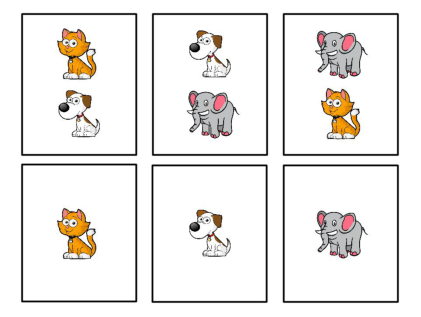
\includegraphics{figs/stimuli-1} 

}

\caption{Cards used in the connective guessing game.}\label{fig:stimuli}
\end{figure}

The study used six cards with cartoon images of a cat, a dog, and an
elephant (Figure \ref{fig:stimuli}). There were two types of cards:
cards with only one animal and cards with two animals. There were three
types of guesses: simple (e.g. \emph{There is a cat}), conjunctive (e.g.
\emph{There is a cat and a dog}), and disjunctive (e.g. \emph{There is a
cat or a dog}). In each guess, the animal labels used in the guess and
the animal images on the card could have no overlap (e.g.~Image: dog,
Guess: \emph{There is a cat or an elephant}), partial overlap
(e.g.~Image: Cat, Guess: \emph{There is a cat or an elephant}), or total
overlap (e.g.~Image: cat and elephant, Guess: \emph{There is a cat or an
elephant}). Crossing the number of animals on the card, the types of
guesses, and the overlap between the guess and the card yields 12
different possible trial types. I chose 8 trial types (Figure
\ref{fig:trials}), to balance the number of one-animal vs.~two-animal
cards, simple vs.~connective guesses, and expected true vs.~false
trials.

\begin{figure}[t]

{\centering 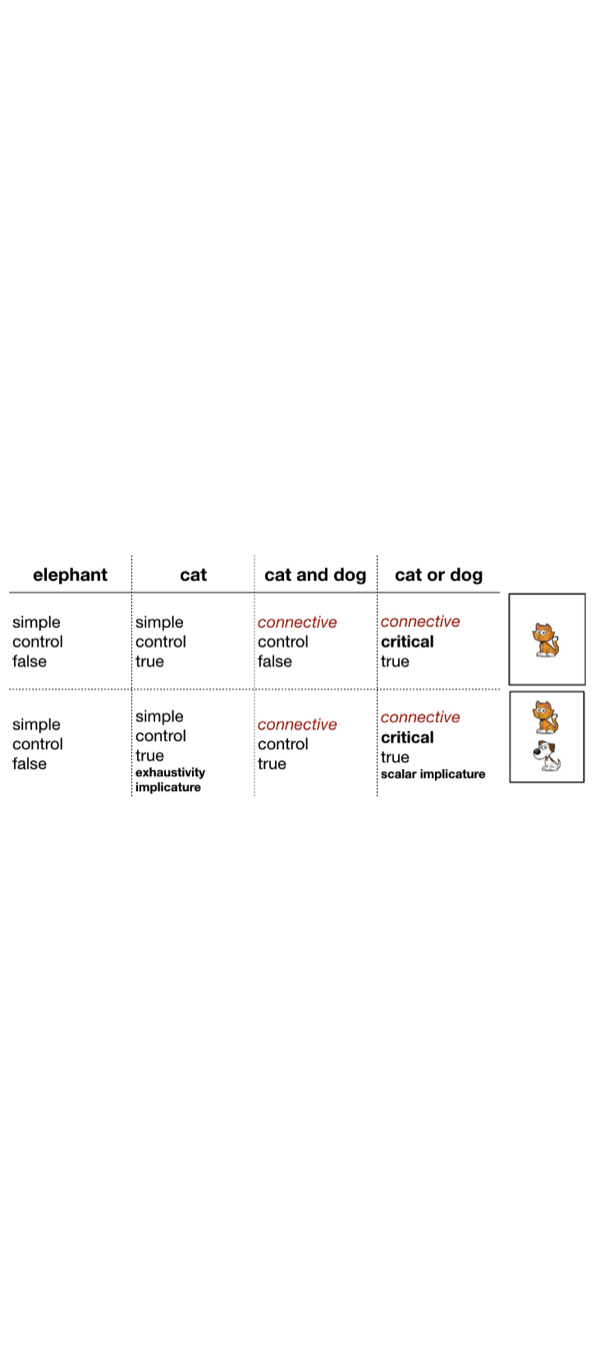
\includegraphics{figs/trials-1} 

}

\caption{Trial types represented by example cards and example guesses.}\label{fig:trials}
\end{figure}

\paragraph{Participants and Procedure}\label{participants-and-procedure}

\begin{figure}[t]

{\centering 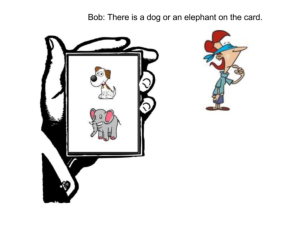
\includegraphics{figs/exampleTrial-1} 

}

\caption{An example trial in Study 1.}\label{fig:exampleTrial}
\end{figure}

I used Amazon's Mechanical Turk (MTurk) for recruitment and the online
platform Qualtrics for data collection and survey design. The task took
about 5 minutes on average to complete. 109 English speaking adults
participated. 57 of them were assigned to a 2AFC judgment task and 52 to
a 3AFC judgment task. In the 2AFC task, participants had to judge using
the options \enquote{wrong} and \enquote{right}. In the 3AFC task they
had to choose between \enquote{wrong}, \enquote{kinda right}, and
\enquote{right}. The two conditions were otherwise identical. There are
many possible labels for the middle option \enquote{kinda right},
including \enquote{kinda wrong} or \enquote{neither}. In a later
experiment (not reported in this dissertation) I tested different
intermediate labels and found that adults consider \enquote{kinda right}
to be the most suitable option for capturing pragmatic infelicity
(Jasbi, Waldon, \& Degen, submitted). I expect similar behavior from
labels like \enquote{a bit right} and \enquote{a little right} which
refer to non-maximal degrees of being right.

The experiment had three phases: introduction, instruction, and test. In
the introduction, participants saw the six cards and read that they
would play a guessing game. Then a blindfolded cartoon character named
Bob appeared on the screen. Participants were told that in each round of
the game, they would see a card and Bob was going to guess what animal
was on the card. I emphasized that Bob could not see anything. I asked
participants to judge whether Bob's guess was right. In the instruction
phase, participants saw an example trial where a card with the image of
a dog was shown with the following sentence written above Bob's head:
\emph{There is a cat on the card}. All participants, who correctly
responded with \enquote{wrong}, proceeded to the test phase.

In the test phase, participants saw one trial per trial type. Within
each trial type, the specific card-guess scenario was chosen at random.
The order of trial types was also randomized. At the end of the study,
participants received \$0.4 as compensation. Figure
\ref{fig:exampleTrial} shows an example test trial.

\begin{longtable}[]{@{}lllll@{}}
\caption{\label{tab:study1info} Summary of Study 1 Methods}\tabularnewline
\toprule
Study & N & Age & Mode & Response Options\tabularnewline
\midrule
\endfirsthead
\toprule
Study & N & Age & Mode & Response Options\tabularnewline
\midrule
\endhead
Study 1 - Part 1 & 57 & Adults & Online (Mturk) & Wrong,
Right\tabularnewline
Study 1 - Part 2 & 52 & Adults & Online (Mturk) & Wrong, Kinda Right,
Right\tabularnewline
\bottomrule
\end{longtable}

\subsubsection{Results}\label{results}

In this section, I first present the results of the 2AFC and 3AFC tasks
with adults. Then I discuss how these results can be interpreted with
respect to the semantics and pragmatics of disjunction in the context of
the guessing game.

\paragraph{Judgments with Two Alternatives
(2AFC)}\label{judgments-with-two-alternatives-2afc}

\begin{figure}[t]

{\centering 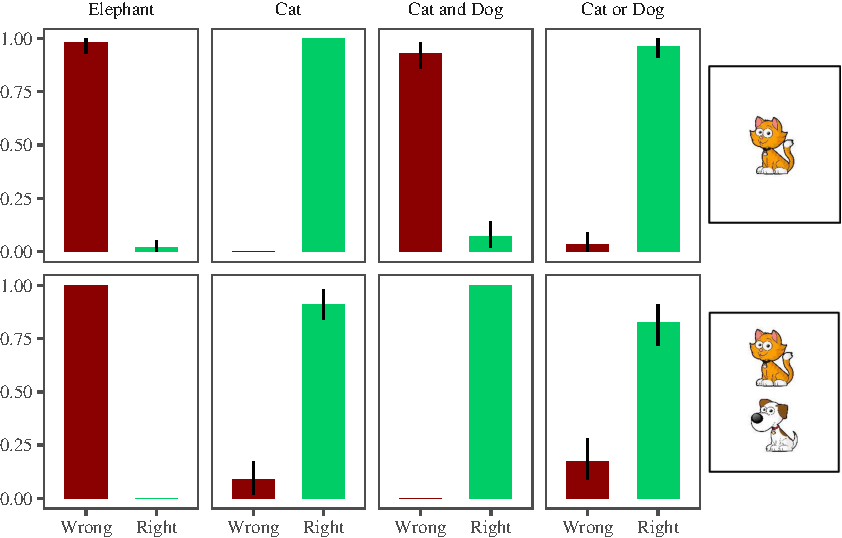
\includegraphics{figs/binaryAdultsPlot-1} 

}

\caption{Adults' two-alternative forced choice judgments.}\label{fig:binaryAdultsPlot}
\end{figure}

Figure \ref{fig:binaryAdultsPlot} shows the results for the adult 2AFC
task. The two left columns show the simple guesses and serve as
controls. The results show that if the animal mentioned in the guess was
not on the card (e.g., elephant), participants judged the guess to be
\enquote{wrong}; if the animal was on the card (e.g., cat), participants
judged the guess to be \enquote{right}. The next two columns of Figure
\ref{fig:binaryAdultsPlot} show the results for the test conditions,
namely conjunction and disjunction. They match the expectations for
logical conjunction and (inclusive) disjunction: an \emph{and}-guess
(e.g.~cat and dog) is \enquote{wrong} if only one of the animals is
shown on the card, and \enquote{right} if both are on the card. An
\emph{or}-guess (e.g.~cat or dog) is \enquote{right} whether one or both
animals are depicted on the card.

\paragraph{Judgments with Three Alternatives
(3AFC)}\label{judgments-with-three-alternatives-3afc}

\begin{figure}[t]

{\centering 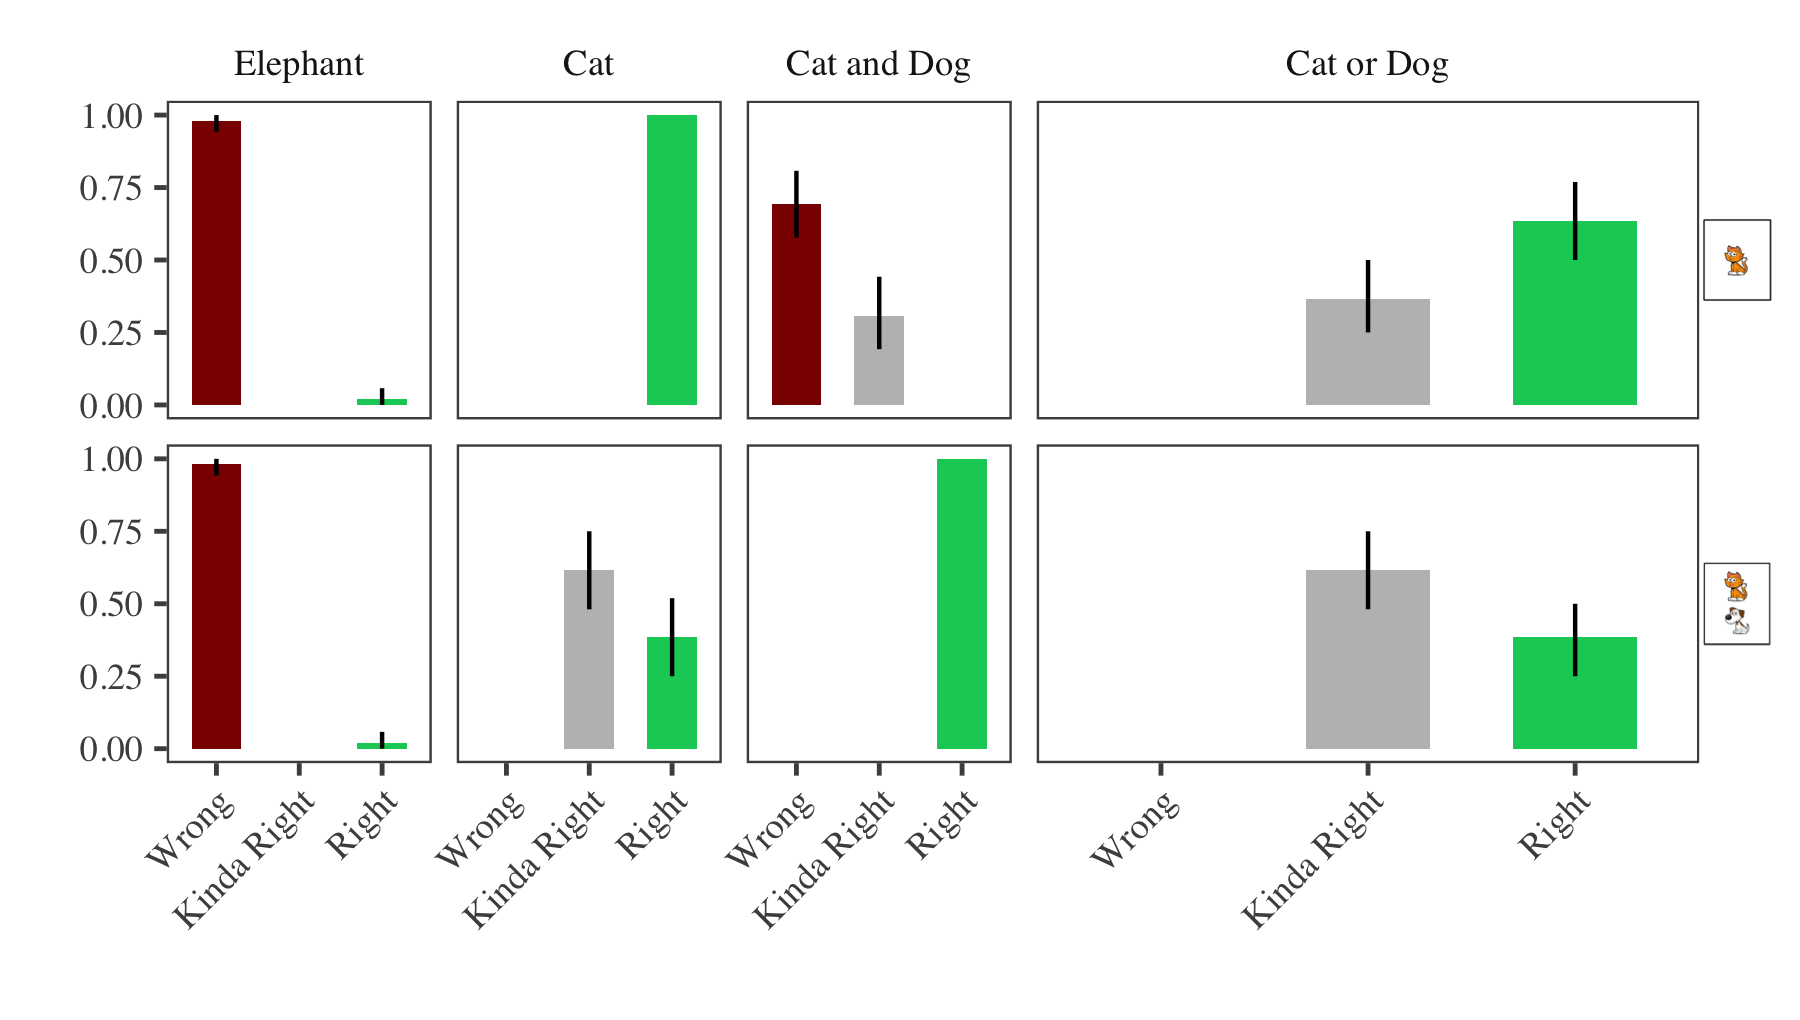
\includegraphics{figs/ternaryAdultsPlot-1} 

}

\caption{Adults' three-alternative forced choice judgments in the connective guessing game.}\label{fig:ternaryAdultsPlot}
\end{figure}

Figure \ref{fig:ternaryAdultsPlot} shows the results for the 3AFC
judgment task. For four trial types, the results are identical to the
2AFC task: if the animal mentioned in the guess was not on the card
(e.g.~elephant), participants judged the guess \enquote{wrong}. If the
animal mentioned (e.g.~cat) was the only animal on the card,
participants judged the guess \enquote{right}. Finally, if there were
two animals and the puppet mentioned them using \emph{and} (e.g.~cat and
dog), all participants considered the guess \enquote{right}.

The four remaining trial types showed different patterns of judgments
than the ones in the 2AFC task. If the animal mentioned (e.g.~cat) was
only one of the animals on the card, participant judgments were divided
between \enquote{right} and \enquote{kinda right} (See Table
\ref{tab:binomStats}, row 1 for the statistical test). Also, most adults
considered a conjunctive guess (e.g.~cat and dog) \enquote{wrong}, when
only one of the animals was on the card (Table \ref{tab:binomStats}, row
2). However, some considered it \enquote{kinda right}, perhaps
suggesting that the intermediate option was used to express the notion
of \enquote{partial truth}. When both animals were on the card everyone
agreed that the conjunctive guess was \enquote{right}.

With respect to disjunctive guesses like \enquote{cat or dog}, if the
card had only one of the animals, most adults considers the guess
\enquote{right} while some considered it \enquote{kinda right} (Table
\ref{tab:binomStats}, row 3). It is possible that the adults who
considered such guesses \enquote{kinda right} were sensitive to the
under-informative nature of a disjunctive guess when a simple guess like
\enquote{cat} would have been more appropriate. If both animals were on
the card, adults were split between \enquote{kinda right} and
\enquote{right} responses (Table \ref{tab:binomStats}, row 4). The
choice of \enquote{kinda right} over \enquote{right} in such trials can
be interpreted as a sign that adults were sensitive to the infelicity of
a disjunction when conjunction was more appropriate. However, the scalar
reasoning with \emph{and} and \emph{or} is subtle and in section
\ref{implicature}, I discuss the nature of this reasoning in the context
of this guessing game.

\begin{longtable}[]{@{}lllllll@{}}
\caption{\label{tab:binomStats} Exact One-Sided Binomial
Test}\tabularnewline
\toprule
\begin{minipage}[b]{0.23\columnwidth}\raggedright\strut
Trial Type\strut
\end{minipage} & \begin{minipage}[b]{0.19\columnwidth}\raggedright\strut
\(n_{_{right}}/n_{_{total}}\)\strut
\end{minipage} & \begin{minipage}[b]{0.08\columnwidth}\raggedright\strut
\(\hat{p}_{_{right}}\)\strut
\end{minipage} & \begin{minipage}[b]{0.08\columnwidth}\raggedright\strut
\(p_{_{null}}\)\strut
\end{minipage} & \begin{minipage}[b]{0.08\columnwidth}\raggedright\strut
P-value\strut
\end{minipage} & \begin{minipage}[b]{0.08\columnwidth}\raggedright\strut
\(95\%~CI\)\strut
\end{minipage} & \begin{minipage}[b]{0.08\columnwidth}\raggedright\strut
\strut
\end{minipage}\tabularnewline
\midrule
\endfirsthead
\toprule
\begin{minipage}[b]{0.23\columnwidth}\raggedright\strut
Trial Type\strut
\end{minipage} & \begin{minipage}[b]{0.19\columnwidth}\raggedright\strut
\(n_{_{right}}/n_{_{total}}\)\strut
\end{minipage} & \begin{minipage}[b]{0.08\columnwidth}\raggedright\strut
\(\hat{p}_{_{right}}\)\strut
\end{minipage} & \begin{minipage}[b]{0.08\columnwidth}\raggedright\strut
\(p_{_{null}}\)\strut
\end{minipage} & \begin{minipage}[b]{0.08\columnwidth}\raggedright\strut
P-value\strut
\end{minipage} & \begin{minipage}[b]{0.08\columnwidth}\raggedright\strut
\(95\%~CI\)\strut
\end{minipage} & \begin{minipage}[b]{0.08\columnwidth}\raggedright\strut
\strut
\end{minipage}\tabularnewline
\midrule
\endhead
\begin{minipage}[t]{0.23\columnwidth}\raggedright\strut
Two Animals - Simple\strut
\end{minipage} & \begin{minipage}[t]{0.19\columnwidth}\raggedright\strut
32/52\strut
\end{minipage} & \begin{minipage}[t]{0.08\columnwidth}\raggedright\strut
0.62\strut
\end{minipage} & \begin{minipage}[t]{0.08\columnwidth}\raggedright\strut
0.50\strut
\end{minipage} & \begin{minipage}[t]{0.08\columnwidth}\raggedright\strut
0.06\strut
\end{minipage} & \begin{minipage}[t]{0.08\columnwidth}\raggedright\strut
0.49-1\strut
\end{minipage} & \begin{minipage}[t]{0.08\columnwidth}\raggedright\strut
\strut
\end{minipage}\tabularnewline
\begin{minipage}[t]{0.23\columnwidth}\raggedright\strut
One Animal - AND\strut
\end{minipage} & \begin{minipage}[t]{0.19\columnwidth}\raggedright\strut
16/52\strut
\end{minipage} & \begin{minipage}[t]{0.08\columnwidth}\raggedright\strut
0.69\strut
\end{minipage} & \begin{minipage}[t]{0.08\columnwidth}\raggedright\strut
0.50\strut
\end{minipage} & \begin{minipage}[t]{0.08\columnwidth}\raggedright\strut
0.00\strut
\end{minipage} & \begin{minipage}[t]{0.08\columnwidth}\raggedright\strut
0.57-1\strut
\end{minipage} & \begin{minipage}[t]{0.08\columnwidth}\raggedright\strut
\strut
\end{minipage}\tabularnewline
\begin{minipage}[t]{0.23\columnwidth}\raggedright\strut
One Animal - OR\strut
\end{minipage} & \begin{minipage}[t]{0.19\columnwidth}\raggedright\strut
19/52\strut
\end{minipage} & \begin{minipage}[t]{0.08\columnwidth}\raggedright\strut
0.63\strut
\end{minipage} & \begin{minipage}[t]{0.08\columnwidth}\raggedright\strut
0.50\strut
\end{minipage} & \begin{minipage}[t]{0.08\columnwidth}\raggedright\strut
0.04\strut
\end{minipage} & \begin{minipage}[t]{0.08\columnwidth}\raggedright\strut
0.51-1\strut
\end{minipage} & \begin{minipage}[t]{0.08\columnwidth}\raggedright\strut
\strut
\end{minipage}\tabularnewline
\begin{minipage}[t]{0.23\columnwidth}\raggedright\strut
Two Animals - OR\strut
\end{minipage} & \begin{minipage}[t]{0.19\columnwidth}\raggedright\strut
32/52\strut
\end{minipage} & \begin{minipage}[t]{0.08\columnwidth}\raggedright\strut
0.62\strut
\end{minipage} & \begin{minipage}[t]{0.08\columnwidth}\raggedright\strut
0.50\strut
\end{minipage} & \begin{minipage}[t]{0.08\columnwidth}\raggedright\strut
0.06\strut
\end{minipage} & \begin{minipage}[t]{0.08\columnwidth}\raggedright\strut
0.49-1\strut
\end{minipage} & \begin{minipage}[t]{0.08\columnwidth}\raggedright\strut
\strut
\end{minipage}\tabularnewline
\bottomrule
\end{longtable}

\subsubsection{Discussion}\label{discussion}

The example sentences bellow show the common interpretations of
conjunctive and disjunctive assertions (Aloni, 2016).

\begin{itemize}
\tightlist
\item
  Bob is sad \emph{and} angry.

  \begin{itemize}
  \tightlist
  \item
    Both are true. (Truth Conditional Meaning)
  \end{itemize}
\item
  Bob is sad \emph{or} angry.

  \begin{itemize}
  \tightlist
  \item
    At least one of the two is true. (Truth Conditional Meaning)
  \item
    Speaker doesn't know which is true. (Ignorance Inference)
  \item
    At most one of the two is true. (Exclusivity Inference)
  \end{itemize}
\end{itemize}

A conjunctive assertion implies that both propositions are true while a
disjunctive assertion implies that at least one is true. These two
inferences follow from the classical truth-conditional account of
conjunction and disjunction. They constitute the semantics of \emph{and}
and \emph{or}. However, a disjunctive assertion often has two additional
inferences: an ignorance inference and an exclusivity inference. These
additional inferences are often classified under pragmatic meaning. This
section discusses the semantics and pragmatics of \emph{and} and
\emph{or} in the context of the guessing game in Study 1.\footnote{See
  Gutzmann (2014) for a comprehensive discussion of the definitions and
  boundaries of semantics and pragmatics. Here my definitions and
  assumptions are close to those of Gazdar (1979).}

\paragraph{The Semantics of AND and
OR}\label{the-semantics-of-and-and-or}

Let's assume that the semantics of \emph{and} and \emph{or} in simple
declarative sentences like \enquote{there is a cat or(and) a dog} is
captured by the logical operators conjunction and inclusive disjunction
respectively. A conjunction is true when both conjuncts are true and
false otherwise. An inclusive disjunction is true when at least one
disjunct is true and false otherwise. Let's also assume a simple linking
function in which false statements are judged as \enquote{wrong} and
true statements as \enquote{right} (see Jasbi et al. (submitted) for a
discussion of linking assumptions in this task). In the context of study
1, this purely semantic (i.e.~truth-conditional) account has two main
predictions: 1. Conjunctive guesses like \enquote{cat and dog} are wrong
when only one of the animals is on the card. 2. Disjunctive guesses are
always right because in all such trials at least one of the animals is
present on the card. Figure \ref{fig:binaryAdultsPlot} shows that in
2AFC judgments, both predictions are borne out. In other words,
judgments with two alternatives seem to match the predictions of a
purely semantic account of the connectives \emph{and} and \emph{or} with
a linking function that considers \enquote{right} and \enquote{wrong}
roughly as \enquote{true} and \enquote{false}.

However, in the 3AFC task, judgments deviated from a purely semantic
account in four trial types: 1. disjunction trials with one animal 2.
disjunction trials with two animals, 3. conjunction trials with one
animal, and 4. trials with simple guesses when two animals were shown on
the card. Participants often used the third option \enquote{kinda right}
in these trial types. Other trial types obtained identical results in
2AFC and 3AFC tasks. The comparison of forced choice judgments with two
and three alternatives suggests that two alternatives better captured
the truth-conditional meaning of the connectives, but underestimated
adult pragmatic reasoning in the guessing game.

\paragraph{The Pragmatics of AND and OR}\label{implicature}

\begin{figure}[t]

{\centering 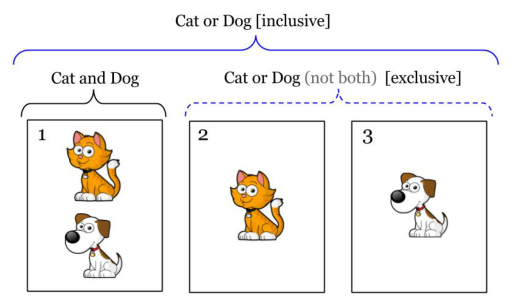
\includegraphics{figs/exclusivity-1} 

}

\caption{Example of cards referred to by a conjunction, inclusive disjunction, and exclusive disjunction.}\label{fig:exclusivity}
\end{figure}

A disjunctive assertion like \enquote{cat or dog} gives rise to an
ignorance inference and an exclusivity inference. The ignorance
inference is the inference that the speaker does not know which disjunct
actually holds. For example in figure \ref{fig:exclusivity}, the
disjunctive guess is uncertain between three outcomes: cards 1, 2, and
3. As pointed out in Chapter \ref{sempragLit}, a disjunction is
infelicitous when the outcome is known to discourse participants. For
example, Tarski mentioned that a disjunction like \enquote{the grass is
green or blue} is odd because we already know that it is green. The
guessing game in this study controls for this ignorance effect by
keeping the guesser blindfolded. Therefore, all the disjunctive guesses
are evaluated in a context where participants know that the guesser is
ignorant of the animals on the cards - both the number of them on the
card and their identity. The exclusivity inference is the inference that
only one of the disjuncts holds and \textbf{not both}. In figure
\ref{fig:exclusivity}, a disjunction like \enquote{cat or dog} only
refers to cards 2 and 3 if it is accompanied by an exclusivity
inference.

Since Grice (1989), this exclusive interpretation of \emph{or} has been
(at least partly) attributed to pragmatic reasoning about the speaker's
connective choice. The reasoning goes like this: conversational
participants are required to make their utterances as informative as
possible. In the context of making predictions and guessing, a guesser
is required to make any guess as specific (i.e.~informative) as
possible.\footnote{When you ask someone to predict the outcome of a coin
  toss, a guess like \enquote{it will be heads or tails} does not count
  as a felicitous guess or prediction, presumably because it will always
  be true.} A conjunction is more specific and informative than a
disjunction (Horn, 1989). For example in Figure \ref{fig:exclusivity},
\enquote{cat and dog} picks card 1 while \enquote{cat or dog} refers to
cards 1, 2, and 3. If speakers intend to refer to card 1, they should
use \emph{and} and say \enquote{cat and dog}. If they use \emph{or}
instead of \emph{and}, they probably do not intend to refer to card 1.
Following this line of reasoning, I can exclude the possibility that a
speaker intends to refer to card 1. The term \enquote{exclusivity
implicature} captures this pragmatic reasoning that results in excluding
the possibility of both disjuncts being true.

My goal here is to lay out the structure of pragmatic reasoning in the
experimental setup and explain how it is manifested in the results of
the experimental studies. There are three main components to the
pragmatic reasoning in the guessing game: 1. the assumptions of the
game. 2. sensitivity to (under)informativity, and 3. the pragmatic
reasoning about the speaker's choice of connectives. Like Katsos \&
Bishop (2011), I have considered \enquote{sensitivity to
informativeness} as a precondition for \enquote{derivation of scalar
implicatures}. I begin with the assumptions of the guessing game.

\begin{itemize}
\tightlist
\item
  \textbf{Guessing Game Assumptions}:

  \begin{itemize}
  \tightlist
  \item
    \textbf{Ignorance}: the guesser does not know the number or identity
    of the animals on the card.
  \item
    \textbf{Specificity}: A guesser is required to be as specific as
    possible, ideally referring to a single card.
  \end{itemize}
\end{itemize}

As explained before, ignorance of the guesser was explicit and part of
the instructions in the study. However, specificity was an implicit
assumption\footnote{Making this assumption explicit is both hard for
  young children and almost impossible when disjunctive guesses are
  used. Disjunctive guesses are always underinformative and never pick
  out a specific card.}. All the guesses used in the experiment can pick
a single card except for disjunctive ones. Conjunctive guesses like
\enquote{cat and dog} pick specific cards. The simple ones like
\enquote{cat} can be strengthened pragmatically to mean \enquote{only a
cat}, and pick a specific card. However, Disjunctive ones like
\enquote{cat or dog} pick two cards in their most specific (exclusive)
sense. Therefore, they are always under-informative and violate the
specificity assumption.

\begin{itemize}
\tightlist
\item
  \textbf{Sensitivity to Informativeness}: The guesser said \enquote{cat
  or dog} which is under-informative and picks card 1, 2, and 3.

  \begin{itemize}
  \tightlist
  \item
    \textbf{Violation Assumption}: the guesser is violating the
    specificity requirement.
  \end{itemize}
\end{itemize}

Participants can detect the underinformativity of disjunctive guesses,
notice the violation of specificity, and then decide whether they would
like to tolerate this violation or punish it. It should be pointed out
that it is hard to distinguish between \enquote{tolerating the
specificity violation} and simply revising the specificity assumption of
the game to avoid a violation. For example, participants may assume that
the goal of the game is saying something true about the cards rather
than being as specific as possible. In either case, the prediction is
that adults who tolerate violation or revise specificity would judge
disjunctive guesses as \enquote{right}. However, if participants assume
specificity and decide to not tolerate its violation, they will judge
all disjunctive guesses to have some degree of infelicity. Since an
under-informative guess is still technically correct, participants may
not punish such a guess with a \enquote{wrong} response and prefer an
intermediate option like \enquote{kinda right}. This is what study 1
shows. With two alternatives, not many adults judge infelicity with
disjunctive guesses and there are almost no \enquote{wrong} responses.
With three alternatives, \enquote{kinda right} responses pop up. Adult
responses are split between \enquote{kinda right} and \enquote{right}.

\begin{figure}[tb]

{\centering 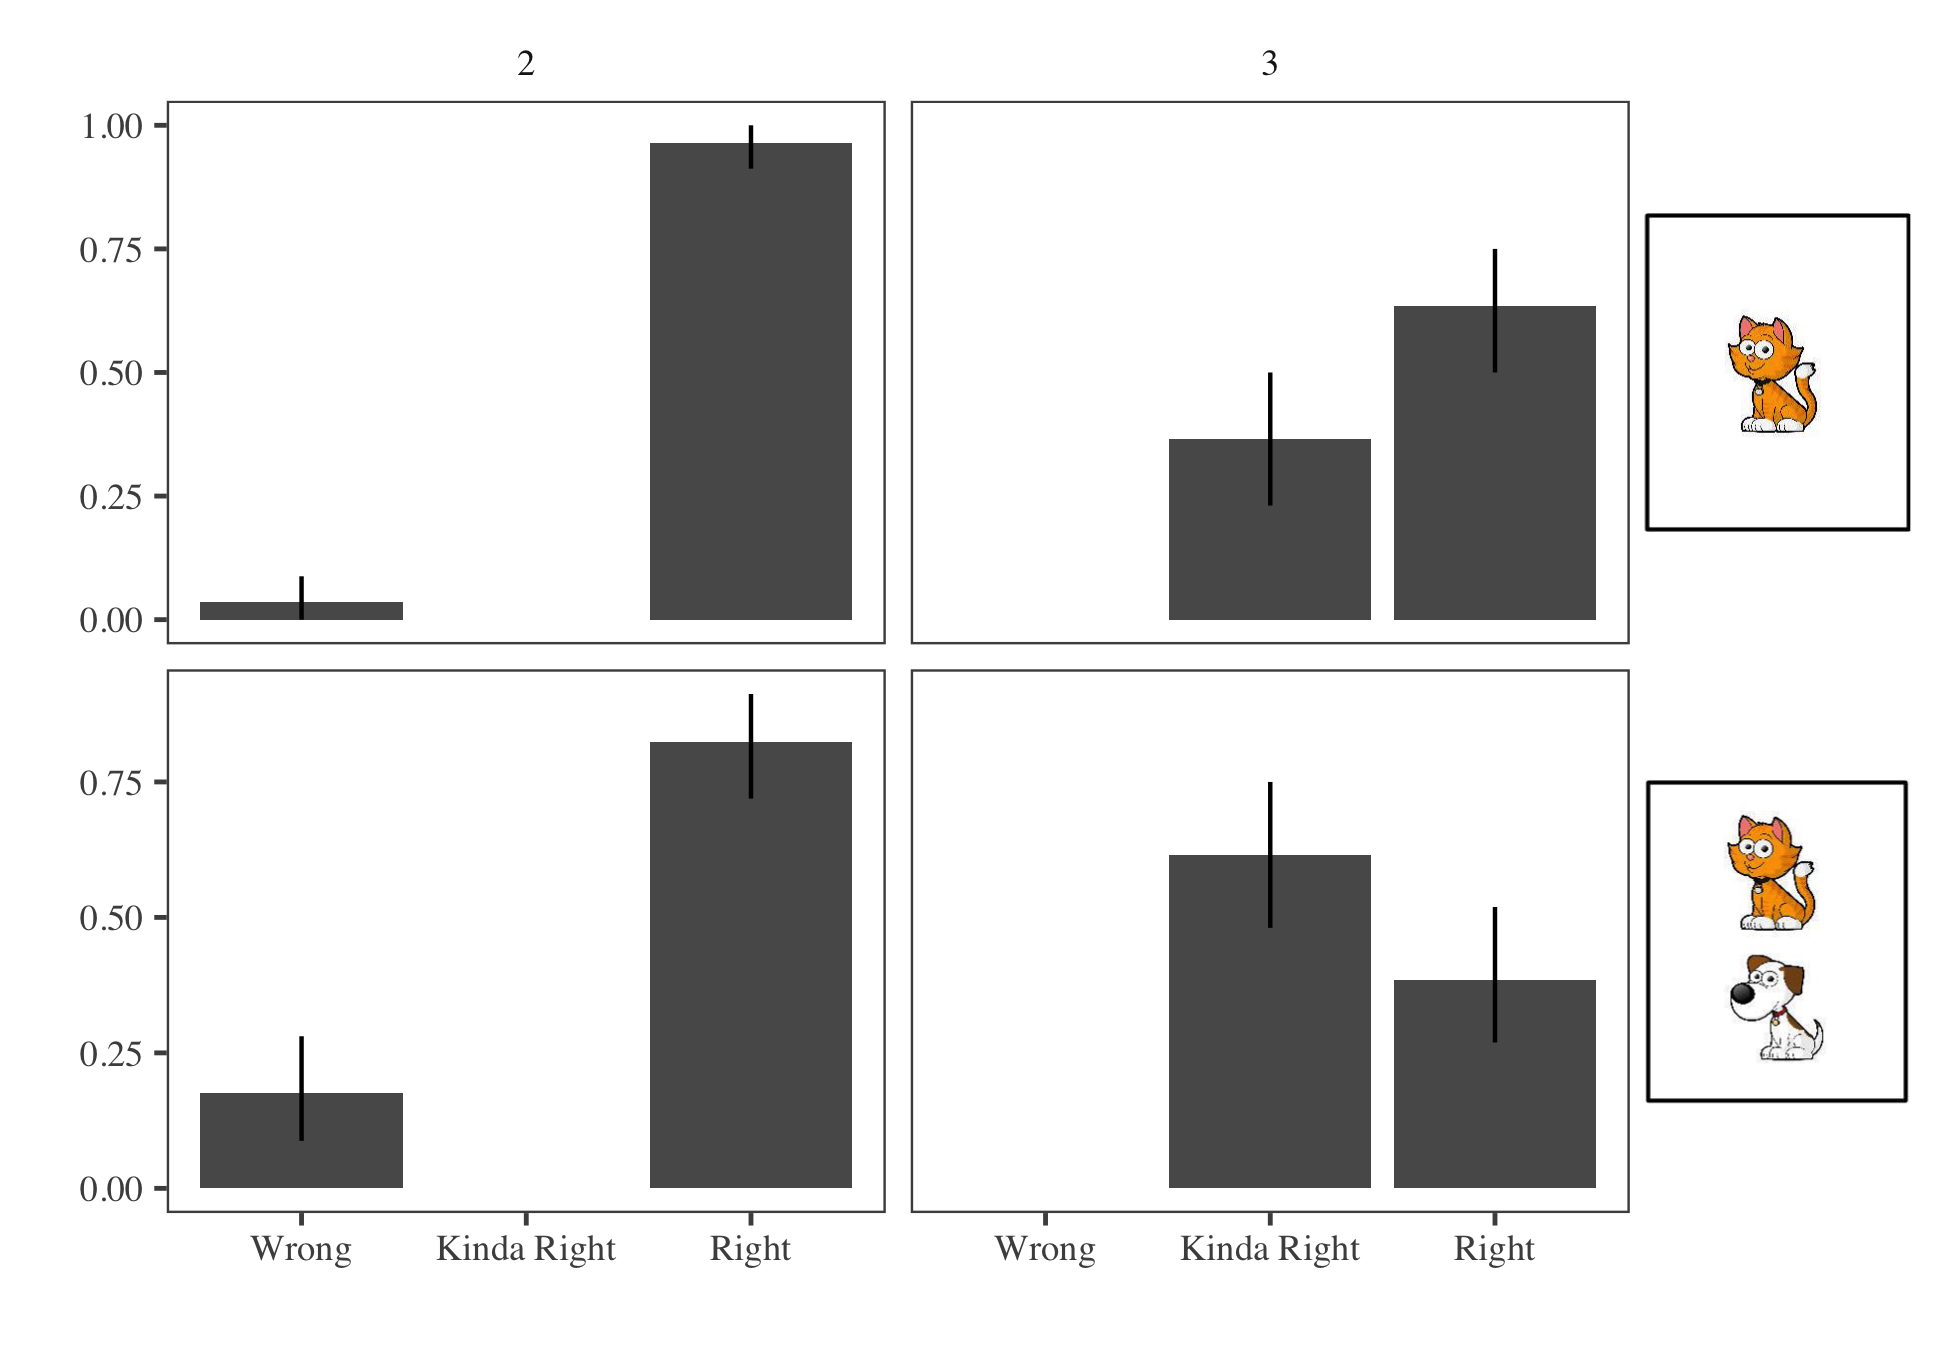
\includegraphics{figs/implicaturePlot-1} 

}

\caption{Adult responses to disjunction guesses like \textit{cat or dog} with 2 and 3 options.}\label{fig:implicaturePlot}
\end{figure}

If detecting and reacting to underinformativity is the whole story, then
disjunctive guesses should show similar degrees of infelicity,
regardless of how many animals there are on the card. However, the
results of the 3AFC task suggest otherwise. A logistic mixed-effects
model with the random intercepts and slopes for subjects and fixed
effect of disjunction type found that when comparing disjunctive guesses
in the 3AFC task, participants were more likely to choose \enquote{kinda
right} than \enquote{right} when both animals were on the card
(\(\beta\)=-1.22, \(z\)=-2.25, \(p\)=0.02). In other words, participants
judged further infelicity with disjunctive guesses that had both
disjuncts as true. Therefore, it is possible that when both disjuncts
were true, some participants went through the following pragmatic
reasoning:

\begin{itemize}
\tightlist
\item
  \textbf{Reasoning on Alternatives}: Why did the guesser choose the
  under-informative connective \emph{or} rather than the more
  informative \emph{and}?

  \begin{itemize}
  \tightlist
  \item
    \textbf{Resolution Assumption}: speaker is trying to be as specific
    as possible by resolving the issue of how many animals are on the
    card.

    \begin{itemize}
    \tightlist
    \item
      \textbf{Exclusivity Implicature}: Given the resolution hypothesis,
      if the speaker had decided that two animals were on the card, they
      should have said \enquote{cat \emph{and} dog}. They did not, so
      they had decided that only one animal is on the card and
      \textbf{not both}.
    \end{itemize}
  \end{itemize}
\end{itemize}

How does the exclusivity implicature affect participant judgments in the
experimental setting? One possibility is that excluding the correct
response pragmatically is treated like cases of excluding the right
response semantically. For example, guessing \enquote{elephant} when
there is a cat on the card. The prediction is that disjunctive trials
with true disjuncts should receive \enquote{wrong} responses. However,
this prediction was not borne out. Such disjunctive trials are almost
never judged as \enquote{wrong}.

Alternatively, it is possible that adults differentiate incorrect
pragmatics from incorrect semantics (i.e.~falsehood) and punish
incorrect pragmatics less than incorrect semantics. This conclusion is
supported by the response patterns across trial types (figure
\ref{fig:ternaryAdultsPlot}). Trial types that received a
\enquote{wrong} response were those that were false. Pragmatically
infelicitous trial types, namely simple guesses like \enquote{cat} or
disjunctive guesses like \enquote{cat or dog} when both animals are on
the card, receive \enquote{kinda right} responses. In other words,
adults consider false utterances as \enquote{wrong} guesses but
infelicitous utterances do not reach the level of being \enquote{wrong};
they are still right even though not completely right. This would
explain why the rates of infelicity (avoiding the \enquote{right}
alternative) differ between 2AFC and 3AFC tasks in disjunctive trials
with true disjuncts (0.18 vs.~0.62).

\subsection{Study 2: Children's three-alternative judgments and
open-ended
feedback}\label{study-2-childrens-three-alternative-judgments-and-open-ended-feedback}

The goal of this study was to examine children's interpretations of
\emph{and} and \emph{or} in the guessing game and compare them to those
of the adults. Since the 3AFC judgment task in study 1 proved better at
capturing the nuances in adults' pragmatic reasoning, I decided to first
test children using three alternatives. I also analyzed children's
open-ended comments about the guesses in the experimental context. Both
three-alternative judgments and the analysis of children's open-ended
responses showed that children differentiate \emph{and} and \emph{or}
statements. The judgment task suggested that children do not consider
disjunctive guesses with true disjuncts as infelicitous. Yet, the
analysis of their open-ended feedback suggests otherwise. Children took
issue with such guesses and corrected them. I conclude that the 3AFC
judgment task may have underestimated children's pragmatic competence.

\subsubsection{Methods}\label{methods-1}

\begin{longtable}[]{@{}lllll@{}}
\caption{\label{tab:study2info} Summary of Study 2 Methods}\tabularnewline
\toprule
\begin{minipage}[b]{0.08\columnwidth}\raggedright\strut
Study\strut
\end{minipage} & \begin{minipage}[b]{0.04\columnwidth}\raggedright\strut
N\strut
\end{minipage} & \begin{minipage}[b]{0.21\columnwidth}\raggedright\strut
Age\strut
\end{minipage} & \begin{minipage}[b]{0.17\columnwidth}\raggedright\strut
Mode\strut
\end{minipage} & \begin{minipage}[b]{0.32\columnwidth}\raggedright\strut
Response Option\strut
\end{minipage}\tabularnewline
\midrule
\endfirsthead
\toprule
\begin{minipage}[b]{0.08\columnwidth}\raggedright\strut
Study\strut
\end{minipage} & \begin{minipage}[b]{0.04\columnwidth}\raggedright\strut
N\strut
\end{minipage} & \begin{minipage}[b]{0.21\columnwidth}\raggedright\strut
Age\strut
\end{minipage} & \begin{minipage}[b]{0.17\columnwidth}\raggedright\strut
Mode\strut
\end{minipage} & \begin{minipage}[b]{0.32\columnwidth}\raggedright\strut
Response Option\strut
\end{minipage}\tabularnewline
\midrule
\endhead
\begin{minipage}[t]{0.08\columnwidth}\raggedright\strut
Study 2\strut
\end{minipage} & \begin{minipage}[t]{0.04\columnwidth}\raggedright\strut
42\strut
\end{minipage} & \begin{minipage}[t]{0.21\columnwidth}\raggedright\strut
3;1-5;2 (M = 4;3)\strut
\end{minipage} & \begin{minipage}[t]{0.17\columnwidth}\raggedright\strut
Study Room\strut
\end{minipage} & \begin{minipage}[t]{0.32\columnwidth}\raggedright\strut
Circle (wrong), Little Star (little right), Big Star (right)\strut
\end{minipage}\tabularnewline
\bottomrule
\end{longtable}

\paragraph{Materials and Design}\label{materials-and-design-1}

I used the same set of cards and linguistic stimuli as the ones in study
1. There were 8 trial types and 2 trials per trial type for a total of
16 trials. I made two changes to make the experiment more suitable for
children. First, instead of the fictional character Bob, a puppet named
Jazzy played the guessing game with them. Jazzy wore a sleeping mask
over his eyes during the game (Figure \ref{fig:jazzy}). Second, a pilot
study showed that a scale with three alternatives is better understood
and used by children if it is presented in the form of rewards to the
puppet rather than verbal responses such as \enquote{wrong}, \enquote{a
little bit right}, and \enquote{right}, or even hand gestures such as
thumbs up, middle, and down. Therefore, I placed a set of red circles,
small blue stars, and big blue stars in front of the children. These
tokens were used to reward the puppet after each guess. During the
introduction, the experimenter explained that if the puppet is right,
the child should give him a big star, if he is a little bit right, a
little star, and if he is not right, a red circle.

\begin{figure}[tb]

{\centering 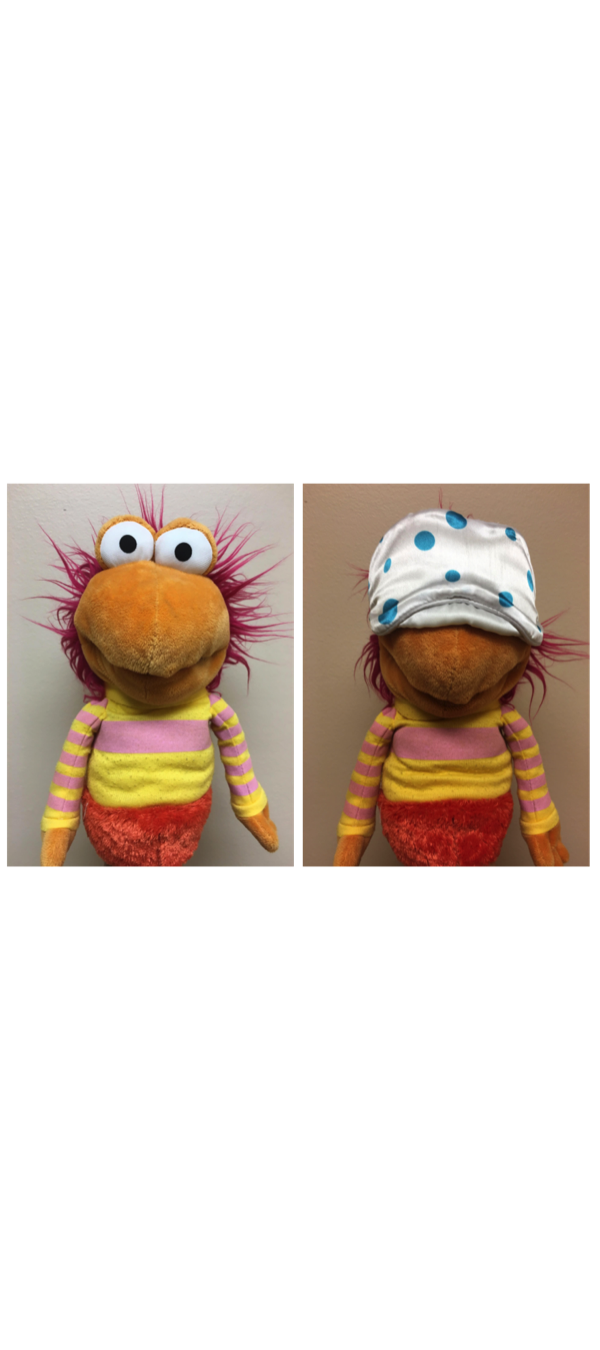
\includegraphics{figs/jazzy-1} 

}

\caption{The puppet, Jazzy, with and without the sleeping mask.}\label{fig:jazzy}
\end{figure}

\paragraph{Participants and
Procedure}\label{participants-and-procedure-1}

I recruited 42 English speaking children from the Bing Nursery School at
Stanford University. Children were between 3;1 and 5;2 years old (Mean =
4;3). The experiment was carried out in a quiet room and all sessions
were videotaped. There was a small table and two chairs in the room.
Children sat on one side of the table and the experimenter and the
puppet on the other side facing the child. The groups of circles, small
stars, and big stars were placed in front of the child from left to
right. A deck of six cards was in front of the experimenter. As in study
1 with adults, the children went through three phases: introduction,
instruction, and test.

The goal of the introduction was for the experimenter to show the cards
to the children and make sure they recognized the animals and knew their
names. The experimenter showed the cards to the children and asked them
to label each animal. All children recognized the animals and could
label them correctly. In the instruction phase, children went through
three example trials. The experimenter explained that he was going to
play with Jazzy (the puppet) first, so that the child could learn the
game. He removed the six introduction cards and placed a deck of three
cards face-down on the table. From top to bottom (first to last), the
cards had the following images: cat, elephant, cat and dog. He put the
sleeping mask on the Jazzy's eyes and explained that the puppet is going
to guess what animal is on the cards. He then picked the first card and
asked the puppet: \enquote{\emph{What do you think is on this card?}}
Jazzy replied with \enquote{\emph{There is a dog}}. The experimenter
showed the cat-card to the child and explained that when the puppet is
\enquote{not right} he gets a circle. The pilot study had shown that
some children struggle with understanding the word \enquote{wrong}, so
\enquote{not right} was used instead. He then asked the child to give
the puppet a circle. Rewards were collected by the experimenter and
placed under the table to not distract the child. The second trial
followed the same pattern except that the puppet guessed \enquote{right}
and the experimenter invited the child to give the puppet a big star. In
the final trial, the puppet guessed that there is a cat on the card when
the card had a cat and a dog on it. The experimenter said that the
puppet was \enquote{a little right} and asked the child to give him a
little star.

\begin{longtable}[]{@{}lll@{}}
\caption{\label{tab:instruction} Instruction Trials.}\tabularnewline
\toprule
Card & Guess & Reward\tabularnewline
\midrule
\endfirsthead
\toprule
Card & Guess & Reward\tabularnewline
\midrule
\endhead
CAT & There is a cat! & Circle\tabularnewline
ELEPHANT & There is an elephant! & Big Star\tabularnewline
CAT-DOG & There is a dog! & Little Star\tabularnewline
\bottomrule
\end{longtable}

In the test phase, the experimenter removed the three instruction cards
and placed a deck of 16 randomized cards on the table. The experimenter
explained that it was the child's turn to play with the puppet. The test
phase followed the pattern described in the instruction phase. The
randomization code as well as the details of the methods are in the
online repository for this study at
\href{https://github.com/jasbi/jasbi_dissertation_LearningDisjunction/tree/master/connective_comprehension/study2/0_methods}{https://github.com/jasbi/jasbi\_dissertation\_LearningDisjunction}.

\paragraph{Offline Annotations}\label{feedbackCoding}

During analysis of the videos, children's linguistic feedback to the
puppet after each guess was categorized into four types: 1. None, 2.
Judgments, 3. Descriptions, and 4. Corrections. The first category
referred to cases where children did not say anything and only rewarded
the puppet. Judgments referred to linguistic feedback such as \emph{you
are right!}, \emph{yes}, \emph{nope}, or \emph{you winned}. Such
feedback only expressed judgments and complemented the rewards.
Descriptions were cases that the child simply mentioned what was on the
card: \emph{cat!}, \emph{dog and elephant!}, \emph{There is a cat and a
dog!} etc. Finally, corrections referred to feedback that provided
additional linguistic elements that acted like corrections to what the
puppet had said. Examples include: \emph{Just a cat!}, \emph{Both!},
\emph{The two are!}, \emph{Only cat}, \emph{cat AND dog} (with emphasis
placed on \emph{and}). In trials where the child provided both judgments
as well as descriptions or corrections, I placed the feedback into the
more informative categories, namely description or correction.

\subsubsection{Results}\label{results-1}

\begin{figure}[t]

{\centering 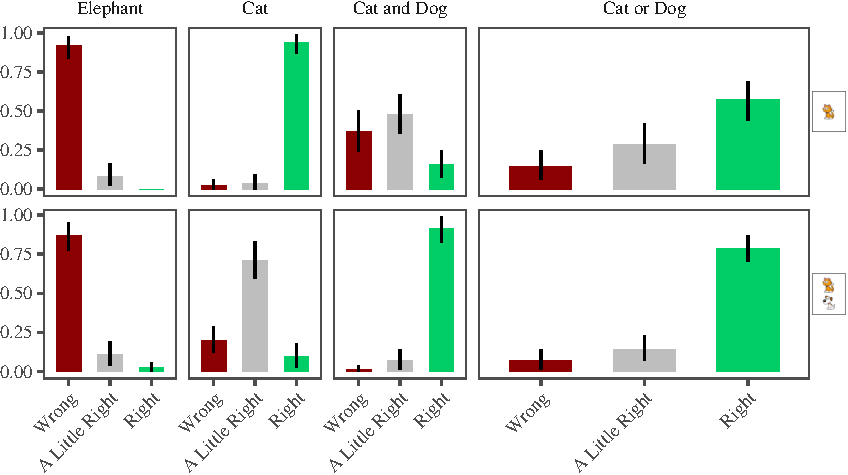
\includegraphics{figs/childrenTernaryPlot-1} 

}

\caption{Children's ternary judgments in the connective guessing game.}\label{fig:childrenTernaryPlot}
\end{figure}

Figure \ref{fig:childrenTernaryPlot} shows the results for children's
3AFC judgments. Starting from the left column, if the mentioned animal
was not on the card (e.g.~elephant), children judged the guess as
\enquote{wrong}. If the animal mentioned (e.g.~cat) was the only animal
on the card, children judged the guess to be \enquote{right}. Here I
will ignore the results for trial types in which the animal mentioned
was one of the animals on the card. The reason is that such trials were
used in the instruction phase to introduce the \enquote{little bit
right} guesses, and the results are potentially biased by the
instructions.

In conjunctive guesses (e.g. \emph{cat and dog}), when only one of the
animals mentioned was on the card, children judged the guess as
\enquote{wrong} or \enquote{a little bit right}. However, if both
animals were on the card, they judged the conjunctive guess as
\enquote{right}. In disjunctive guesses (e.g. \emph{cat or dog}), when
only one of the animals mentioned was on the card, children considered
the guess \enquote{right} or \enquote{kinda right}. If both animals were
on the card, the disjunctive guess was considered \enquote{right}.

The comparison of conjunction and disjunction trials (last two columns
of figure \ref{fig:childrenTernaryPlot}) shows that overall, children
distinguished between \emph{and} and \emph{or} when one animal was on
the card. Given that the one-animal conjunction trials are false but the
one-animal disjunction trials are true, the difference in response
patterns may suggest that children understood the truth-conditional
differences between \emph{and} and \emph{or}. The truth judgments did
not provide evidence that children differentiated \emph{and} and
\emph{or} when two animals were on the card. Since in the majority of
examples with \emph{or} and two animals, children responded with
\enquote{right}, it is possible to conclude from the judgment data that
children did not generate exclusivity inferences in this task.

Figure \ref{fig:childAdultComp} compares the results for children and
adults' 3AFC judgments in the conjunction and disjunction trials. The
major difference between adults and children's responses was disjunctive
trials with two animals on the card. Most children considered such
trials as \enquote{right} while adults considered them as \enquote{kinda
right} or \enquote{right}. In the next section, I use Bayesian
regression modeling to compare adults' and children's three-alternative
responses more systematically.

\begin{figure}[t]

{\centering 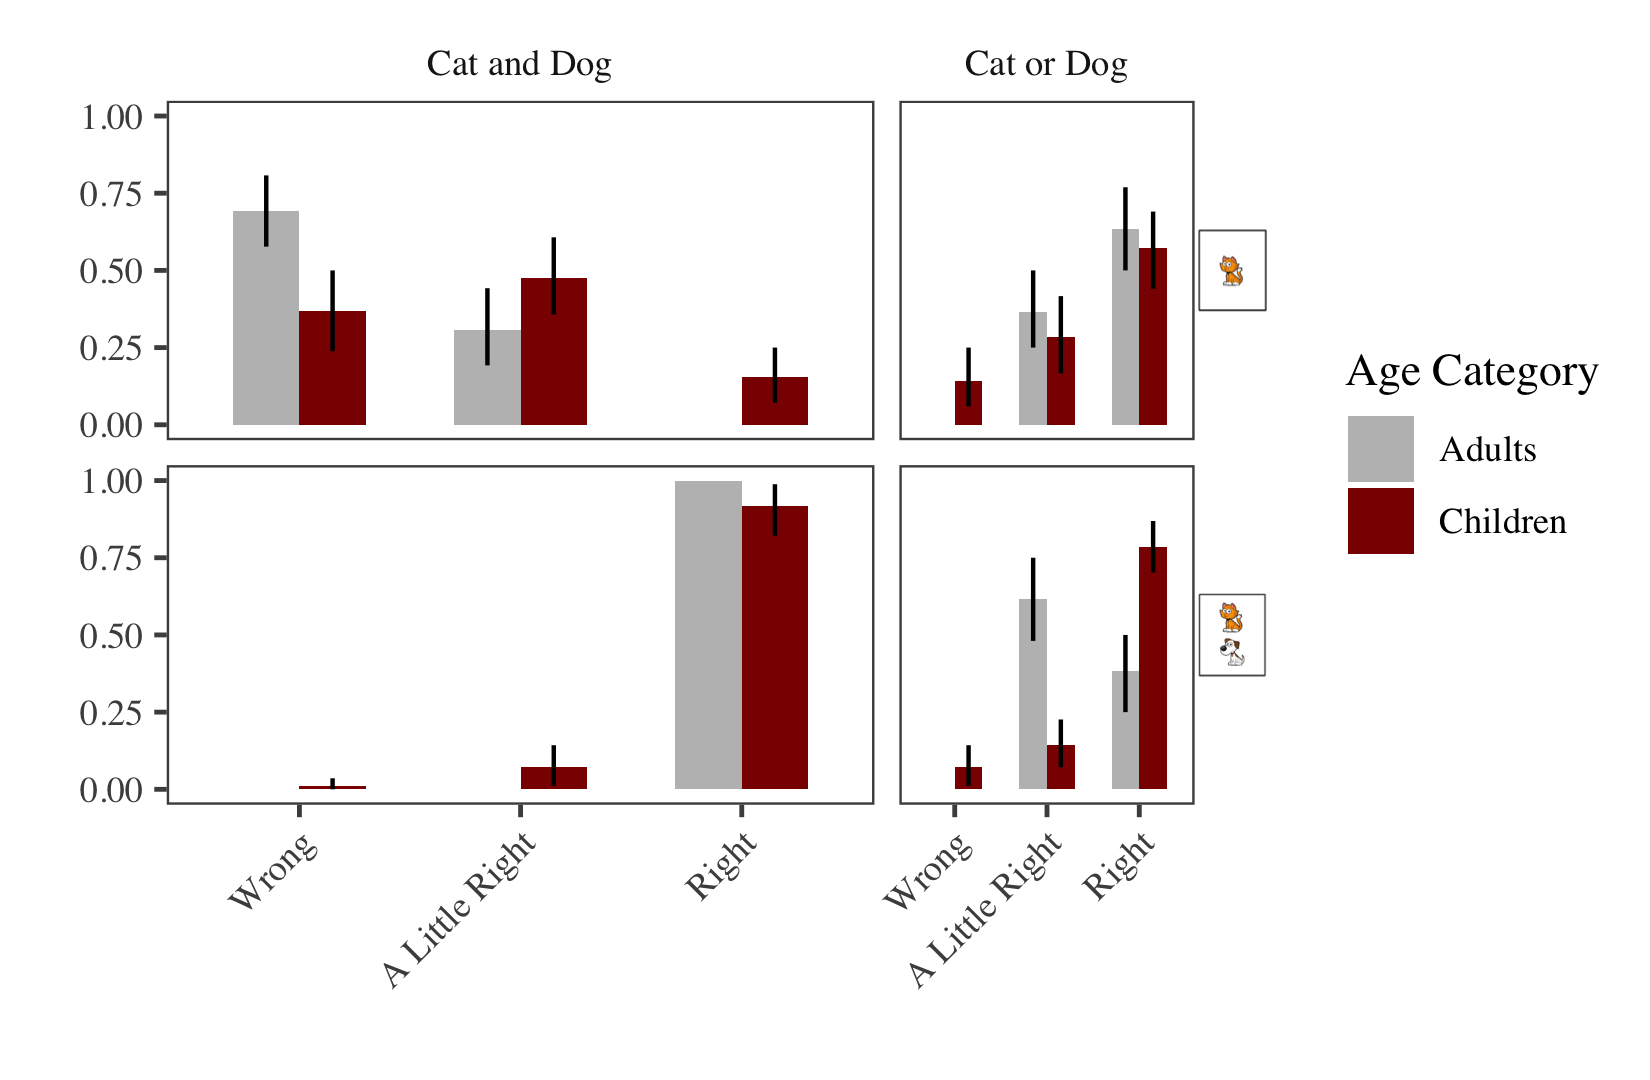
\includegraphics{figs/childAdultComp-1} 

}

\caption{Comparison of Adults' and Children's ternary judgments.}\label{fig:childAdultComp}
\end{figure}

\paragraph{Analysis and Statistical
Modeling}\label{analysis-and-statistical-modeling}

\begin{figure}[t]

{\centering 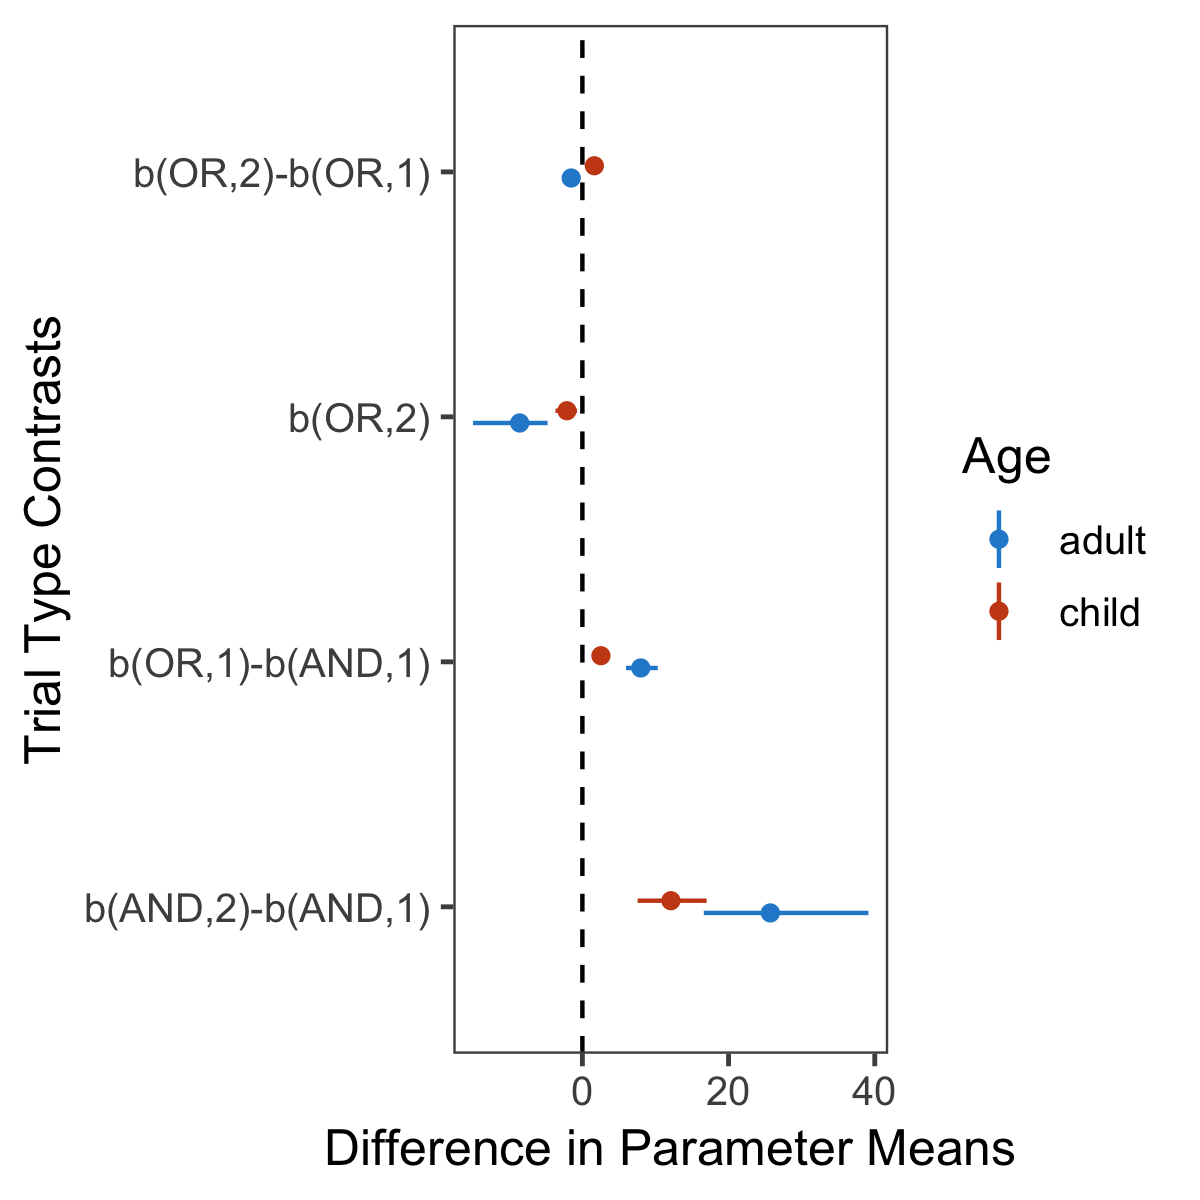
\includegraphics{figs/stanModelPlot-1} 

}

\caption{Coefficients capturing the relevant comparisons across conditions in ternary judgments in Study 1 and 2. In naming the coefficients like b(OR,2), OR/AND represents the connective used and the number 1/2 represents the number of animals on the card. Error bars represent 99\% regions of highest posterior density.}\label{fig:stanModelPlot}
\end{figure}

I used the R package RStan for Bayesian statistical modeling to fit
separate ordinal mixed-effects logistic models for the children's and
adults' judgments. The response variable had three ordered levels:
\emph{wrong}, \emph{kinda right}, and \emph{right}. The trial types
\emph{One-Animal-OR}, \emph{Two-Animals-OR}, \emph{One-Animal-AND}
constituted the (dummy-coded) fixed effects of the model with
\emph{Two-Animals-AND} set as the intercept. The model also included
by-subject random intercepts. The priors over trial types and the random
intercepts were set to \(\mathcal{N}(0,10)\). I also included parameters
\(C_1\) and \(C_2\), the two cutpoints delimiting the logistic for 1)
\emph{wrong} and \emph{kinda right} and 2) \emph{kinda right} and
\emph{right} responses, drawn with the prior
\(\mathcal{N}(0,1)\).\footnote{I used a tight prior in this case to
  decrease posterior correlations between cutpoints and intercept.} All
four chains converged after 3000 samples (with a burn-in period of 1500
samples).

I made inferences based on the highest-posterior density (HPD) intervals
for the coefficients estimated from each model. Because predictors are
dummy-coded, it's possible to examine contrasts of interest by computing
the difference between coefficients for pairs of conditions I wish to
contrast. In naming the coefficients like b(OR,2), OR/AND represents the
connective used and the number represents the number of animals on the
card. Figure \ref{fig:stanModelPlot} shows the contrasts of interest:
\emph{b(OR, 2)-b(OR,1)} represents the difference between the estimated
coefficients for the disjunction trials with two animal on the card and
those with only one; \emph{b(OR, 2)} represents the difference between
the estimated coefficients for the conjunction trials with two animals
and the disjunction trials with two animals; and so on.

Overall, adults' and children's estimated coefficients are similar in
sign to one another, though adults' are more extreme. In the conjunction
trials (\emph{b(AND, 2)-b(AND,1)}), children and adults showed a strong
preference for the cards with two animals rather than one. At the same
time, given two animals on the card, children and adults showed a
preference for \emph{and} rather than \emph{or} (\emph{b(OR, 2)}).
However, with only one animal on the card, children and adults preferred
a disjunctive guess (\emph{b(OR, 1)-b(AND,1)}). These results are
compatible with the truth conditions of conjunction and disjunction.

The main difference between adults and children shows up in the contrast
between the disjunctive trial types: two animals vs.~only one
(\emph{b(OR, 2)-b(OR,1)}). On average, children rated disjunction trials
with two animals higher than those with only one. Adults on the other
hand showed the opposite pattern: they rated disjunction trials with two
animals lower. This pattern is compatible with current accounts of
pragmatic development that suggest an absence of implicatures in
children's interpretations. The idea is that while adults strengthen the
disjunctive guess \enquote{cat or dog} to \enquote{cat or dog but not
both}, children simply interpret it as \enquote{cat or dog or both}.
Adults are therefore going to rate trials with both disjuncts true
lower.

The slight preference children show for cards with two animals when the
guess is disjunctive is also compatible with the account proposed by
Singh et al. (2016) and Tieu et al. (2016). However, the effect is much
smaller here than was reported in their studies. The comparison with
conjunction trials makes it clear that overall, children are not
interpreting \emph{or} as having a conjunctive meaning. The effect in
this study can be more accurately described as a preference in judgment
for both disjuncts being true rather than a conjunctive interpretation
of disjunction. The results from children's spontaneous linguistic
feedback make it less likely that children interpretive \emph{or} as a
conjunction. I will discuss this issue further in section
\ref{conjunctive}.

\paragraph{Children's open-ended
feedback}\label{childrens-open-ended-feedback}

\begin{longtable}[]{@{}lll@{}}
\caption{\label{tab:feedbackCat} Definitions and Examples for the Feedback
Categories.}\tabularnewline
\toprule
\begin{minipage}[b]{0.11\columnwidth}\raggedright\strut
Category\strut
\end{minipage} & \begin{minipage}[b]{0.46\columnwidth}\raggedright\strut
Definition\strut
\end{minipage} & \begin{minipage}[b]{0.32\columnwidth}\raggedright\strut
Examples\strut
\end{minipage}\tabularnewline
\midrule
\endfirsthead
\toprule
\begin{minipage}[b]{0.11\columnwidth}\raggedright\strut
Category\strut
\end{minipage} & \begin{minipage}[b]{0.46\columnwidth}\raggedright\strut
Definition\strut
\end{minipage} & \begin{minipage}[b]{0.32\columnwidth}\raggedright\strut
Examples\strut
\end{minipage}\tabularnewline
\midrule
\endhead
\begin{minipage}[t]{0.11\columnwidth}\raggedright\strut
None\strut
\end{minipage} & \begin{minipage}[t]{0.46\columnwidth}\raggedright\strut
no feedback provided to the puppet, only reward\strut
\end{minipage} & \begin{minipage}[t]{0.32\columnwidth}\raggedright\strut
\strut
\end{minipage}\tabularnewline
\begin{minipage}[t]{0.11\columnwidth}\raggedright\strut
Judgment\strut
\end{minipage} & \begin{minipage}[t]{0.46\columnwidth}\raggedright\strut
the child said yes/no, you are right, etc.\strut
\end{minipage} & \begin{minipage}[t]{0.32\columnwidth}\raggedright\strut
\enquote{No!} , \enquote{You are right Jazzy!}\strut
\end{minipage}\tabularnewline
\begin{minipage}[t]{0.11\columnwidth}\raggedright\strut
Description\strut
\end{minipage} & \begin{minipage}[t]{0.46\columnwidth}\raggedright\strut
mentioned the animal(s) on the card\strut
\end{minipage} & \begin{minipage}[t]{0.32\columnwidth}\raggedright\strut
\enquote{elephant}, \enquote{cat and dog}\strut
\end{minipage}\tabularnewline
\begin{minipage}[t]{0.11\columnwidth}\raggedright\strut
Correction\strut
\end{minipage} & \begin{minipage}[t]{0.46\columnwidth}\raggedright\strut
used focus particles like \emph{only}/\emph{just}, emphasized \emph{and}
or used \emph{both}\strut
\end{minipage} & \begin{minipage}[t]{0.32\columnwidth}\raggedright\strut
\enquote{only cat}, \enquote{just elephant}, \enquote{both!},
\enquote{cat AND dog!}\strut
\end{minipage}\tabularnewline
\bottomrule
\end{longtable}

As explained in section \ref{feedbackCoding}, I also categorized and
annotated children's spontaneous and free form verbal reactions to the
puppet's guesses. Table \ref{tab:feedbackCat} summarizes the definitions
and examples for each category and Figure \ref{fig:feedbackData} shows
the results.

\begin{figure}[h]

{\centering 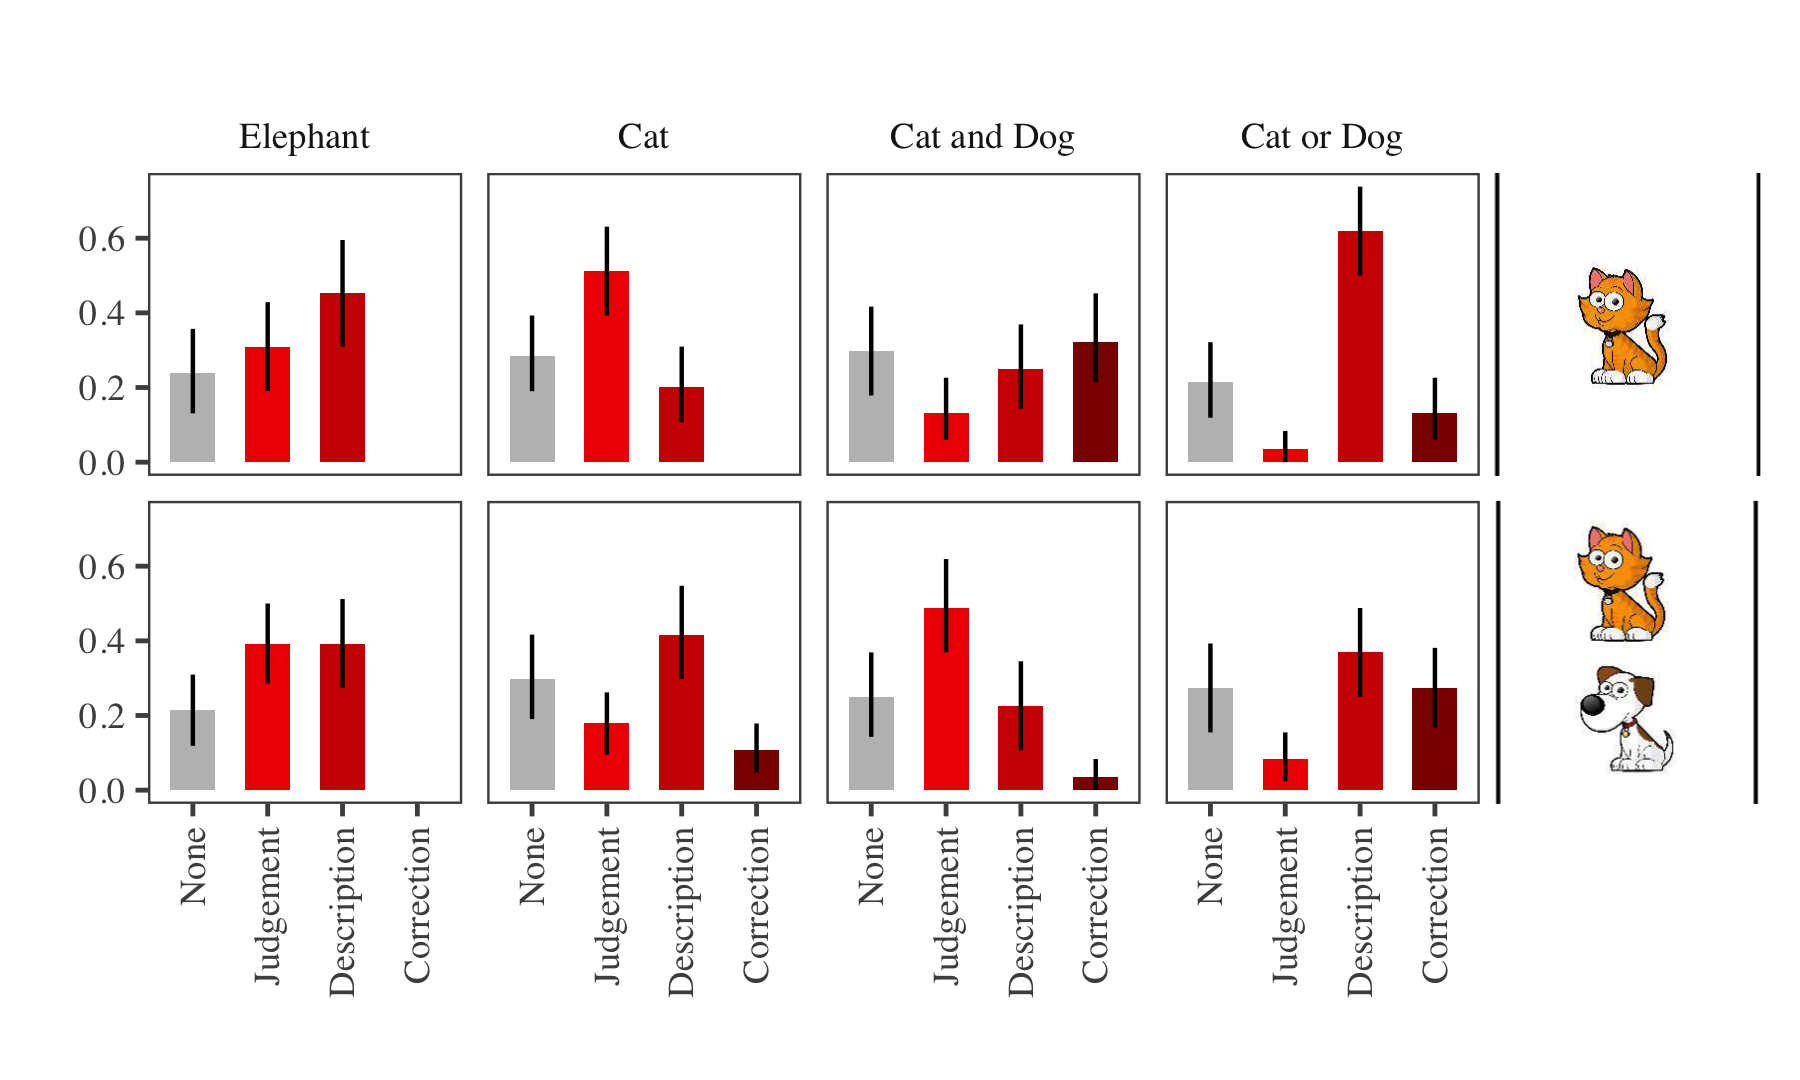
\includegraphics{figs/feedbackData-1} 

}

\caption{Children's open-ended Feedback. Error bars represent 95\% confidence intervals.}\label{fig:feedbackData}
\end{figure}

I should first point out that each trial type has a similar number of
\enquote{None} cases, for feedback. Some children remained more or less
silent throughout the experiment and only provided rewards to the
puppet. In the next study I focus on children's open-ended feedback. In
the discussion and analysis here I will not comment further on the
\enquote{None} category but focus on the other three categories.

In the leftmost column, when the animal guessed (e.g.~elephant) was not
on the card, children either provided judgments like \enquote{No!} or
described what was on the card like \enquote{cat} or \enquote{cat and
dog}. However, when the animal guessed was the only animal on the card
(e.g.~cat), most children provided a positive judgment like
\enquote{Yes}. When the animal guessed was only one of the animals on
the card, children described what was on the card, say, \enquote{cat and
dog}. Corrections were rare for all these four control trial types.

In the critical trial types with conjunction and disjunction, children
showed a high rate of corrections and description when the guess used
\emph{and} but there was only one animal on the card. In their
corrections, children used the focus particles \emph{just} and
\emph{only} like \enquote{just a cat} or \enquote{only a cat}. However,
in trial types where conjunction was used and both animals were
depicted, children predominantly provided positive judgments like
\enquote{Yes!} and \enquote{You are right}. Considering disjunctive
guesses like \enquote{cat or dog}, when only one of the animals was on
the card, most children simply described what was on the card, for
example \enquote{cat}. However, when both animals were on the card,
children corrected the puppet by saying \emph{both} or emphasizing
\emph{and} as in \enquote{cat AND dog}.

I performed chi-squared goodness-of-fit tests to compare the feedback
distributions in the critical conditions with \emph{and} and \emph{or}.
Here I focus on those trials (the four bar charts on the right of Figure
\ref{fig:feedbackData}). Children's linguistic feedback showed three
patterns. First, the one-animal conjunctive and two-animal disjunctive
(top left and bottom right) trials contained a higher proportion of
Corrections than the other trial types. These were trials where the
guesses were either false or infelicitous. In the conjunction trials, a
comparison of the feedback distribution in one-animal and two-animal
conditions was statistically significant (\(\chi^2\)(3, 83) = 201.65, p
\textless{} .0001), suggesting that children gave different feedback to
true and false guesses. A similar numerical trend was present in the
disjunction trials, but it was not significant (\(\chi^2\)(9, 4) = 12, p
= 0.21).

Second, the one-animal disjunctive trials (top right) showed the highest
proportion of \emph{Descriptions}. These are trials in which the guess
is correct but not specific enough: it leaves two possibilities open.
These trials were significantly different from the one-animal trials for
conjunction (\(\chi^2\)(3, 83) = 62.16, p \textless{} .0001). Finally,
the two-animal conjunctive trials (bottom left) showed the highest
proportion of \emph{Judgments} such as \emph{You are right!}. This was
not surprising given that these trials represented the optimal guessing
scenario. These trials had a significantly different feedback
distribution from the matching disjunction trials (\(\chi^2\)(3, 84) =
184.98, p \textless{} .0001).

\subsubsection{Discussion}\label{discussion-1}

In study 2, I used a 3AFC judgment task to test children's comprehension
of logical connectives \emph{and} and \emph{or}. I compared these
results to those found in the 3AFC judgment task of study 1 with adults.
The general comparison showed that adults and children had similar
patterns of judgments, except when both disjuncts were true. In such
cases, adults judged the disjunctive guess as not completely right while
most children found it completely right. There was even a slight
preference among children to rewarded the puppet more in such cases,
compared to cases of disjunction when only one disjunct was true.

To consider another measure of children's comprehension, I also looked
at children's spontaneous open-ended feedback in response to the
guesses. My analysis suggested that children recognized false and
infelicitous utterances with the connectives and provided appropriate
corrective feedback. As expected from an adult-like understanding of
connectives, children corrected the puppet most often when there was
only one animal on the card and the guess was conjunctive, or when there
were two animals on the card and the guess was disjunctive. Perhaps the
most important finding was that children increased their corrective
feedback in disjunctive guesses where both disjuncts were true, compared
to those with only one true disjunct. These findings differ from the
results of the 3AFC judgment task which suggested that children did not
find any infelicity with disjunctive guesses when both disjuncts were
true.

The analysis of children's open-ended feedback raises two important
issues. First, as I mentioned before, it runs counter to what the 3AFC
judgment task suggests with respect to exclusivity implicatures
(i.e.~trials with disjunction when both disjuncts are true). The
forced-choice judgment task suggests that children find such cases
unproblematic while analysis of their spontaneous feedback shows that
they provided more corrections to the puppet. Second, a common
explanation for why children fail to derive0 implicatures is that they
cannot access the stronger alternative to the disjunction \emph{or},
namely \emph{and} (Barner, Brooks, \& Bale, 2011). However, in the
context of the guessing game, some children explicitly mentioned the
word \emph{and} as what the puppet should have said instead of
\emph{or}. Interestingly, these children continued to reward the puppet
and considered the guess \enquote{right}. This raises the possibility
that children's forced-choice truth value judgments, whether with two or
three alternatives, do not fully reflect their pragmatic knowledge. In
study 3, I used both a 2AFC truth judgment task and an analysis of
children's open-ended feedback. If the findings of study 2 were on the
right track, I expected to replicate the same pattern in study 3: the
analysis of children's spontaneous linguistic feedback provides more
evidence that children are sensitive to pragmatic violations than the
results of the 2AFC judgments.

\subsection{Study 3: Children's 2AFC judgments and open-ended
feedback}\label{study-3-childrens-2afc-judgments-and-open-ended-feedback}

This study used the same paradigm as study 2 but focused on children's
open-ended feedback and aimed at replicating the findings in study 2.
The main hypothesis was that four-year-olds provide corrective feedback
to the puppet if both disjuncts are true, but they do not consider this
infelicity to be grave enough to render the guess itself
\enquote{wrong}. The main hypothesis along with relevant analyses and
predictions were preregistered in an \enquote{As Predicted}
format\footnote{The As Predicted pdf document is accessible at
  \url{https://aspredicted.org/x9ez2.pdf}.}. The study used a 2AFC
judgment task to compare with the open-ended feedback results. The
prediction was that children would provide corrective feedback to the
puppet when both disjuncts were true, yet consider the guess
\enquote{right} and not reflect this infelicity in their truth value
judgments. This is what the study found.

\subsubsection{Methods}\label{methods-2}

\begin{longtable}[]{@{}lllll@{}}
\caption{\label{tab:study3info} Summary of Study 1, 2, and 3
Methods}\tabularnewline
\toprule
\begin{minipage}[b]{0.19\columnwidth}\raggedright\strut
Study\strut
\end{minipage} & \begin{minipage}[b]{0.02\columnwidth}\raggedright\strut
N\strut
\end{minipage} & \begin{minipage}[b]{0.20\columnwidth}\raggedright\strut
Age\strut
\end{minipage} & \begin{minipage}[b]{0.11\columnwidth}\raggedright\strut
Mode\strut
\end{minipage} & \begin{minipage}[b]{0.32\columnwidth}\raggedright\strut
Response Options\strut
\end{minipage}\tabularnewline
\midrule
\endfirsthead
\toprule
\begin{minipage}[b]{0.19\columnwidth}\raggedright\strut
Study\strut
\end{minipage} & \begin{minipage}[b]{0.02\columnwidth}\raggedright\strut
N\strut
\end{minipage} & \begin{minipage}[b]{0.20\columnwidth}\raggedright\strut
Age\strut
\end{minipage} & \begin{minipage}[b]{0.11\columnwidth}\raggedright\strut
Mode\strut
\end{minipage} & \begin{minipage}[b]{0.32\columnwidth}\raggedright\strut
Response Options\strut
\end{minipage}\tabularnewline
\midrule
\endhead
\begin{minipage}[t]{0.19\columnwidth}\raggedright\strut
Study 1 - Part 1\strut
\end{minipage} & \begin{minipage}[t]{0.02\columnwidth}\raggedright\strut
57\strut
\end{minipage} & \begin{minipage}[t]{0.20\columnwidth}\raggedright\strut
Adults\strut
\end{minipage} & \begin{minipage}[t]{0.11\columnwidth}\raggedright\strut
Online (Mturk)\strut
\end{minipage} & \begin{minipage}[t]{0.32\columnwidth}\raggedright\strut
Wrong, Right\strut
\end{minipage}\tabularnewline
\begin{minipage}[t]{0.19\columnwidth}\raggedright\strut
Study 1 - Part 2\strut
\end{minipage} & \begin{minipage}[t]{0.02\columnwidth}\raggedright\strut
52\strut
\end{minipage} & \begin{minipage}[t]{0.20\columnwidth}\raggedright\strut
Adults\strut
\end{minipage} & \begin{minipage}[t]{0.11\columnwidth}\raggedright\strut
Online (Mturk)\strut
\end{minipage} & \begin{minipage}[t]{0.32\columnwidth}\raggedright\strut
Wrong, Kinda Right, Right\strut
\end{minipage}\tabularnewline
\begin{minipage}[t]{0.19\columnwidth}\raggedright\strut
Study 2\strut
\end{minipage} & \begin{minipage}[t]{0.02\columnwidth}\raggedright\strut
42\strut
\end{minipage} & \begin{minipage}[t]{0.20\columnwidth}\raggedright\strut
3;1-5;2 (M = 4;3)\strut
\end{minipage} & \begin{minipage}[t]{0.11\columnwidth}\raggedright\strut
Study Room\strut
\end{minipage} & \begin{minipage}[t]{0.32\columnwidth}\raggedright\strut
Circle (Wrong), Little Star (Little Right), Big Star (Right)\strut
\end{minipage}\tabularnewline
\begin{minipage}[t]{0.19\columnwidth}\raggedright\strut
Study 3\strut
\end{minipage} & \begin{minipage}[t]{0.02\columnwidth}\raggedright\strut
50\strut
\end{minipage} & \begin{minipage}[t]{0.20\columnwidth}\raggedright\strut
3;6-5;9 (M = 4;7)\strut
\end{minipage} & \begin{minipage}[t]{0.11\columnwidth}\raggedright\strut
Study Room\strut
\end{minipage} & \begin{minipage}[t]{0.32\columnwidth}\raggedright\strut
Yes (Right)/No (Wrong) - Open-ended Feedback\strut
\end{minipage}\tabularnewline
\bottomrule
\end{longtable}

\paragraph{Materials and Design}\label{materials-and-design-2}

Study 3 was similar to Study 2 but differed in how children provided
their judgments. Based on the findings in Study 2, I focused on verbal
judgments and feedback, instead of rewards. I used two different ways of
measuring children's judgments. First, I encouraged children to provide
verbal feedback to the puppet. They were asked to say \enquote{yes} when
the puppet was right, and \enquote{no} when he was not. They were also
encouraged to help the puppet say it better when he was not right. After
children were done with this initial open-ended feedback, for each trial
I asked a forced choice yes/no judgment question: \enquote{Was Jazzy
(the puppet) right?}. This question elicited a \enquote{yes} or
\enquote{no} response for each trial independent of their earlier
open-ended response. These two measures allowed me to compare open-ended
and forced-choice judgments.

\paragraph{Participants and
Procedure}\label{participants-and-procedure-2}

I recruited 50 English speaking children from the Bing Nursery School at
Stanford University. Children were between 3;6 and 5;9 years old (Mean =
4;7). The setup and procedure were similar to Study 2, except there were
no rewards on the table. As before, participants sat through three
phases: introduction, instruction, and test. The introduction phase made
sure children knew the names of the animals on the cards. In the
instruction phase, they received four training trials, as shown in Table
\ref{tab:instructionStudy3}.

As in Study 2, the experimenter put a sleeping mask over the puppet's
eyes and explained that Jazzy (the puppet) was going to guess what
animal was on the cards. He then picked the first card and asked the
puppet: \enquote{\emph{What do you think is on this card?}} The puppet
replied with \enquote{\emph{There is a dog}}. The experimenter showed
the cat-card to the child and said: when Jazzy is \emph{not right}, tell
him \enquote{no}. He then asked the child to say \enquote{no} to the
puppet. The second trial followed the same pattern except that the
puppet guessed \emph{right} and the experimenter invited the child to
say \enquote{yes} to the puppet. There were two more instruction trials
before the test phase began. This contained 16 randomized trials, half
of which contained guesses with the words \emph{and} and \emph{or}. The
randomization code as well as the details of the methods are on the
online repository for this dissertation at
\href{https://github.com/jasbi/jasbi_dissertation_LearningDisjunction/blob/master/connective_comprehension/study3/0_methods/children}{https://github.com/jasbi/jasbi\_dissertation\_LearningDisjunction}.

\begin{longtable}[]{@{}lll@{}}
\caption{\label{tab:instructionStudy3} Instruction Trials for Study
3.}\tabularnewline
\toprule
Card & Guess & Response\tabularnewline
\midrule
\endfirsthead
\toprule
Card & Guess & Response\tabularnewline
\midrule
\endhead
CAT & there is a dog! & No!\tabularnewline
ELEPHANT & there is an elephant! & Yes!\tabularnewline
DOG-ELEPHANT & there is a cat! & No!\tabularnewline
DOG & there is a dog! & Yes!\tabularnewline
\bottomrule
\end{longtable}

\subsubsection{Results}\label{results-2}

I first look at the results of the 2AFC judgement task for each trial
type and compare them to those of the adults' in Study 1. Then I analyze
children's open-ended responses and compare them to the forced choice
responses obtained in the same trial types. For the 2AFC judgments I
excluded 26 trials (out of total 800) where children either did not
provide a Yes/No response or provided both (i.e. \enquote{Yes and No}).
The exclusions were almost equally distributed among different types of
guesses and cards. In the analysis of children's open-ended feedback, I
excluded 8 trials (out of total 800) where children either did not
provide any feedback or their feedback could not be categorized into the
existing categories.

\paragraph{Two-Alternative Forced Choice
Judgments}\label{two-alternative-forced-choice-judgments}

\begin{figure}[t]

{\centering 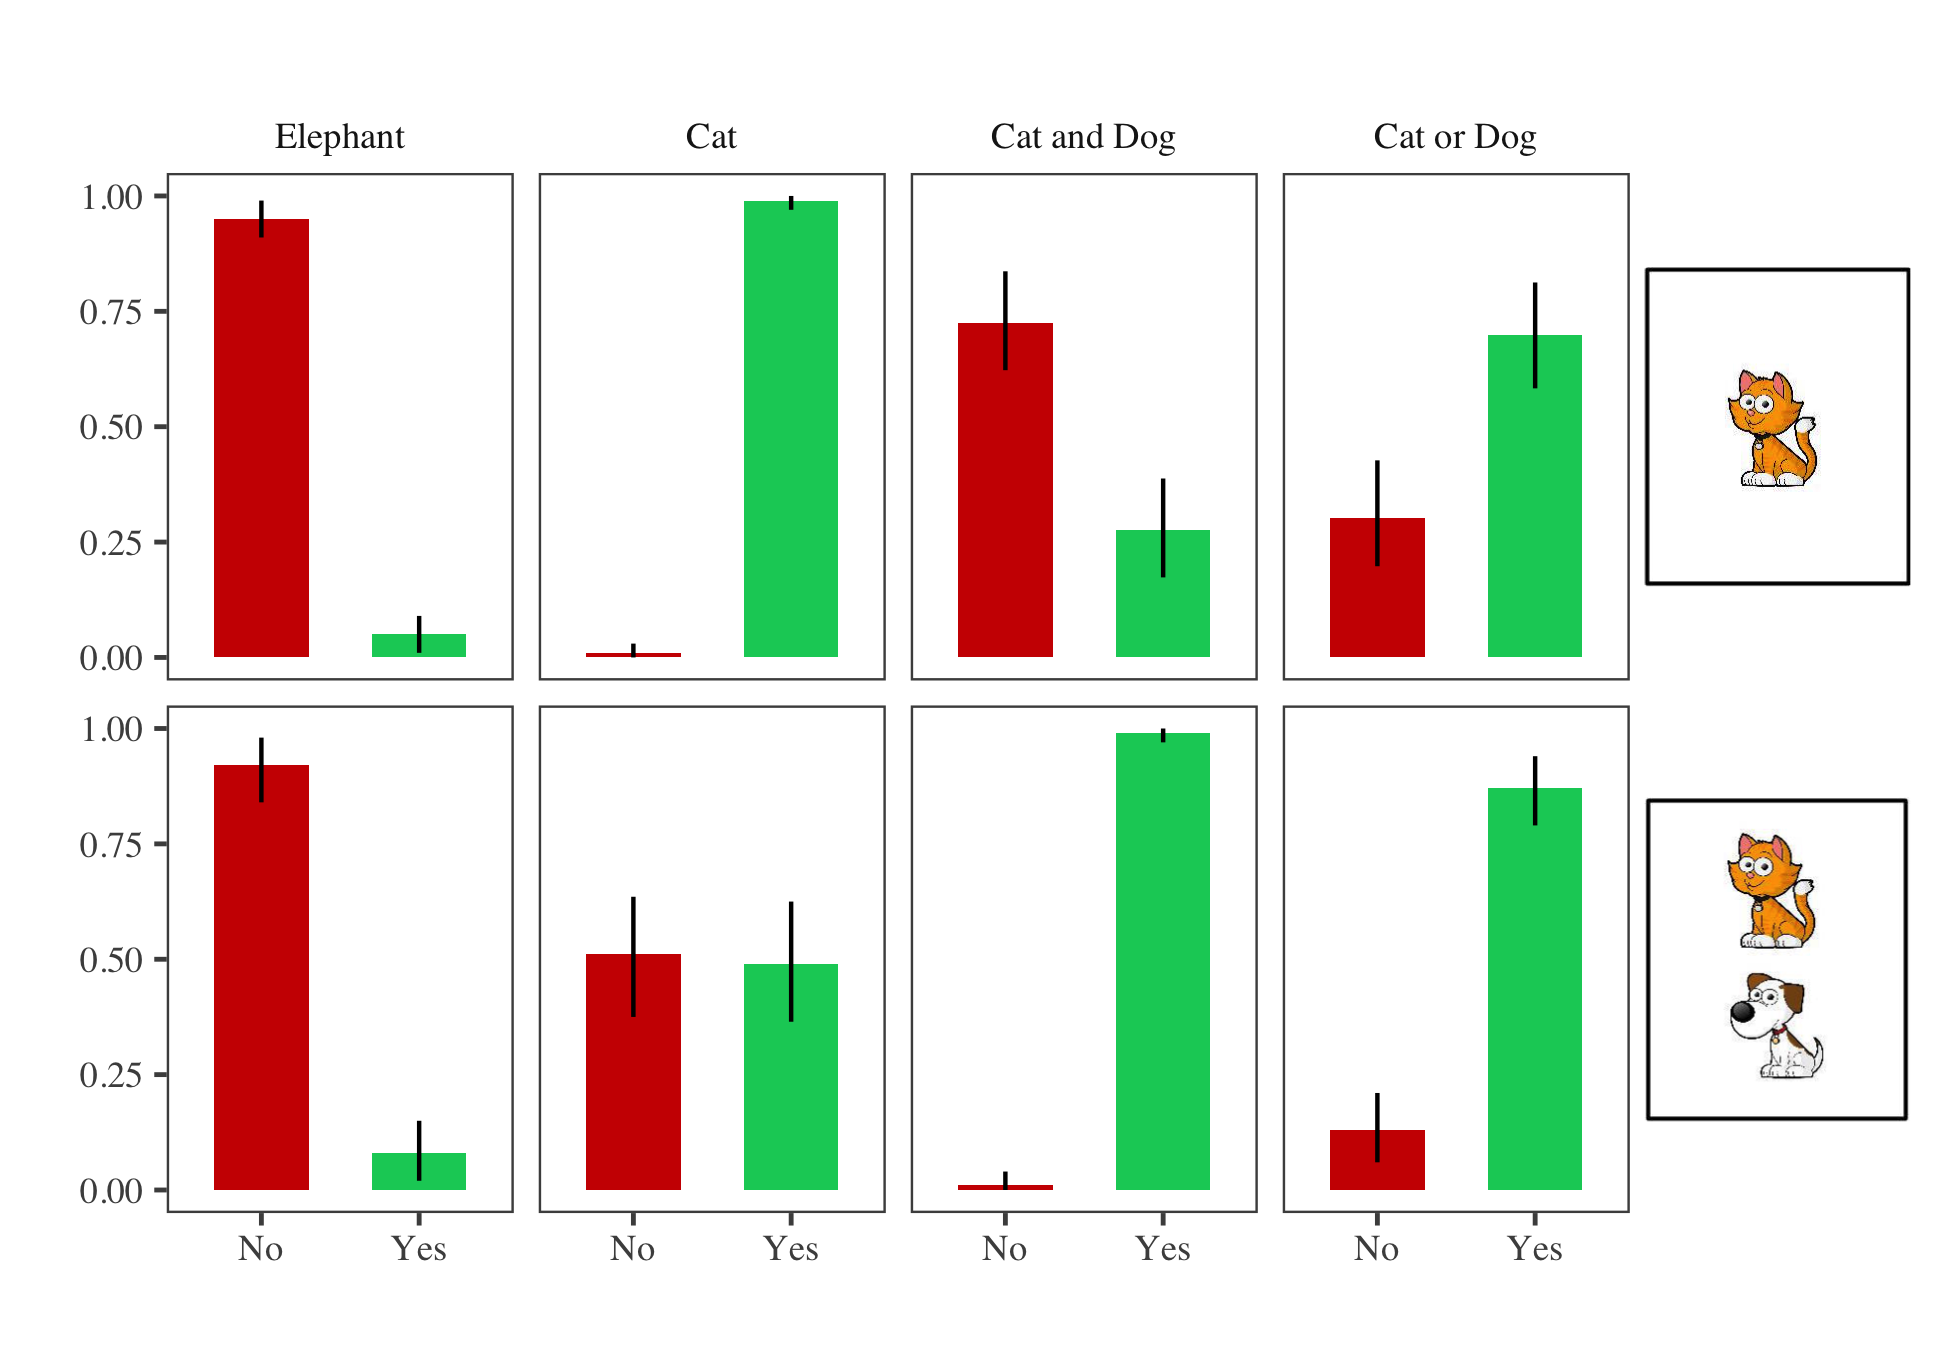
\includegraphics{figs/Study3tvjtPlot-1} 

}

\caption{Children's binary truth value judgments.}\label{fig:Study3tvjtPlot}
\end{figure}

Figure \ref{fig:Study3tvjtPlot} shows children's 2AFC judgments. In the
leftmost column, when the animal guessed was not on the card
(e.g.~elephant), children considered the guess \enquote{wrong}. When the
animal guessed was the only animal on the card (e.g.~cat), children
considered the guess \enquote{right}. However, if the animal guessed
(e.g.~cat) was only one of the animals on the card, children were
equally split between \enquote{wrong} and \enquote{right} judgments. On
the other hand, almost all adults considered such guesses
\enquote{right} in their 2AFC judgments (Figure
\ref{fig:binaryAdultsPlot}). In such trial types, children seem to
interpret the guess \enquote{there is a cat} as \enquote{there is
\textbf{only} a cat}, while adults do not. This difference between
children and adults is unexpected for a theory of meaning acquisition
that assumes children are overall more logical or literal as
interpreters than adults (Noveck, 2001).

In the trials with \emph{and} and \emph{or}, children's judgments were
similar to those of adults. Figure \ref{fig:BinaryPlotComp} compares
adults' and children's 2AFC judgments. In trials with conjunction, when
only one of the animals was on the card, most children considered the
guess \enquote{wrong}. This is similar to adults' judgments, but
different in extent: adults were more consistent and unanimous in
rejecting such guesses. A mixed effects logistic regression with the
fixed effect of age category (adult vs.~child) and random effect of
subject found no significant difference between adults' and children's
responses in such trials (see Table \ref{tab:statsStudy3}, Conjunction -
One Animal).

\begin{longtable}[]{@{}lcccc@{}}
\caption{\label{tab:statsStudy3} Mixed effects logistic models for
conjunction and disjunction trials when only one disjunct was true, in
2AFC judgments of adults and children, using \texttt{glmer} in R's lme4
package. Formula:
\(Response \sim Age Category + (1|Subject)\).}\tabularnewline
\toprule
Trial Data & Coefficient & Standard Error & Z-Value &
P-value\tabularnewline
\midrule
\endfirsthead
\toprule
Trial Data & Coefficient & Standard Error & Z-Value &
P-value\tabularnewline
\midrule
\endhead
Conjunction - One Animal & -2.05 & 2.86 & -0.72 & 0.47\tabularnewline
Disjunction - One Animal & 1.34 & 1.79 & 0.75 & 0.45\tabularnewline
\bottomrule
\end{longtable}

In conjunctive guesses where both animals were on the card, both
children and adults were unanimous in considering the guess
\enquote{right}. In disjunctive trials when only one of the animals was
on the card, most children considered the guess \enquote{right}. This is
again similar to adults but differs from them in extent: adults more
consistently and unanimously judged such guesses as \enquote{right}. Yet
again, a mixed effects logistic regression with the fixed effect of age
(adult vs.~child) and random effect of subject found no significant
difference between adults' and children's responses in such trials (see
Table \ref{tab:statsStudy3}, Disjunction - One Animal). Adults and
children showed almost identical patterns of judgments in trials where
there was two animals on the card and the guess used the connective
\emph{or}. Children and adults did not differ in their rate of rejecting
disjunctive guesses when both disjuncts were true.

\begin{figure}[t]

{\centering 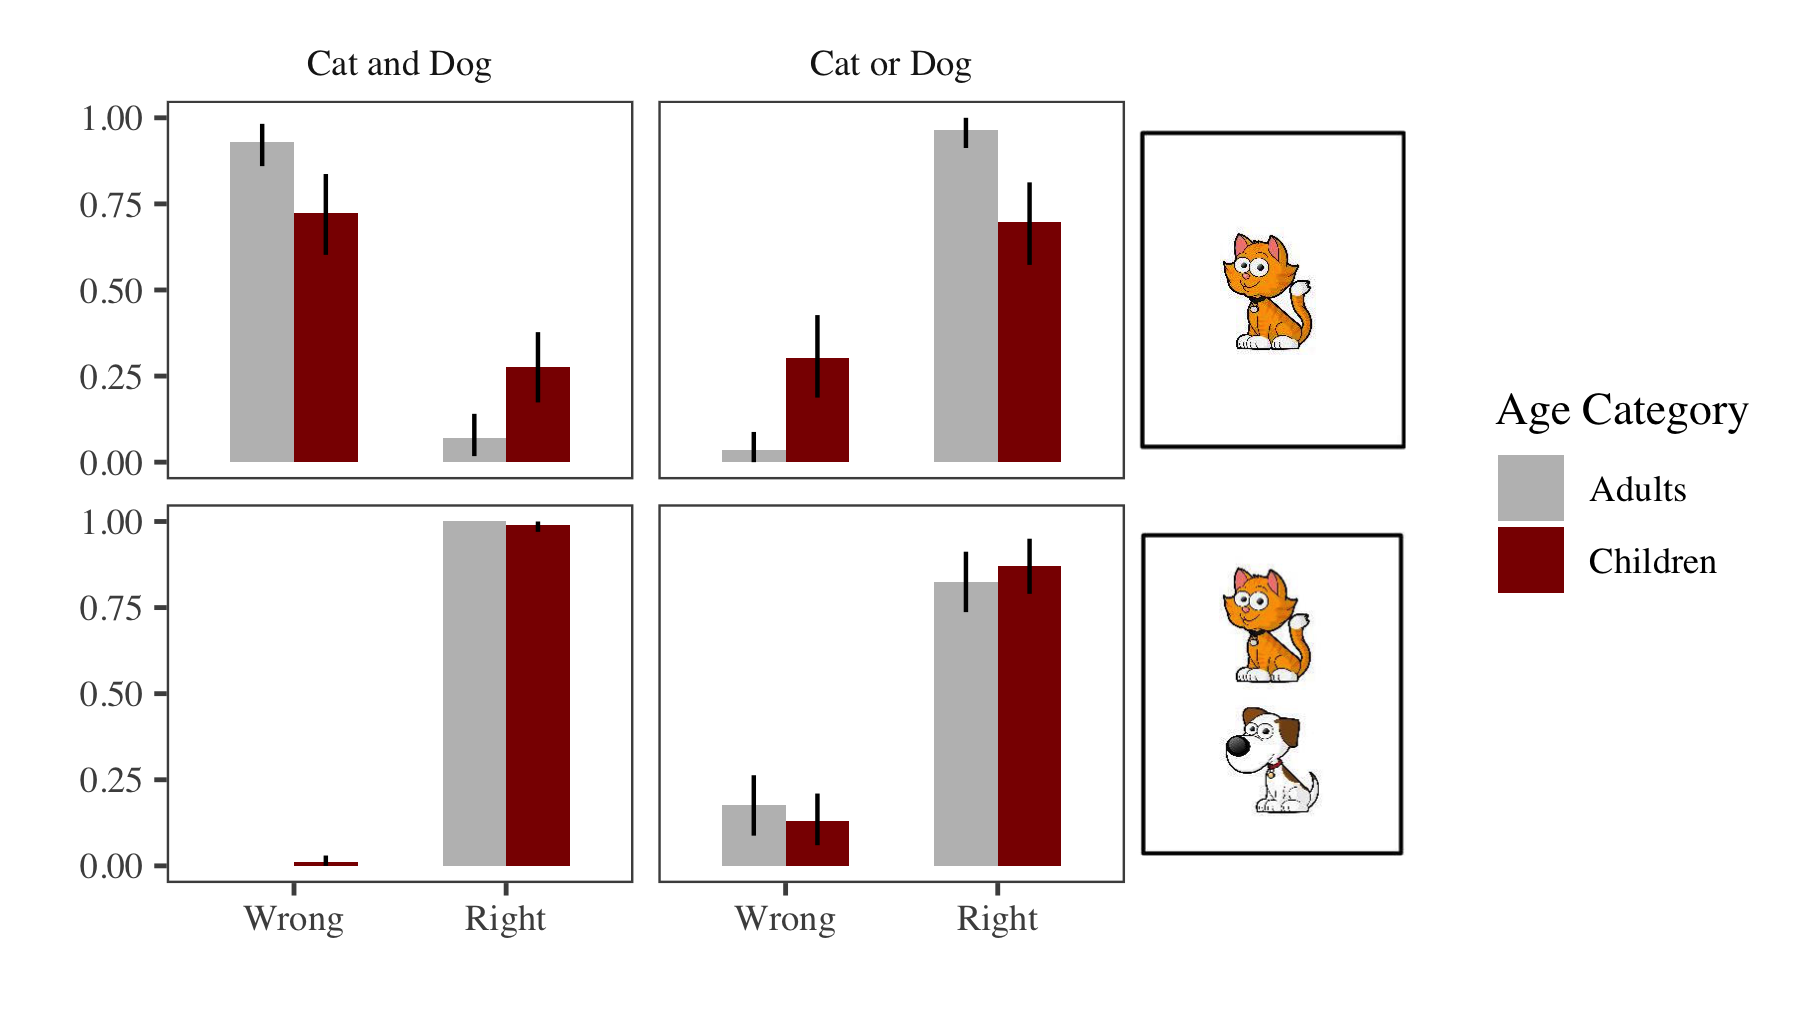
\includegraphics{figs/BinaryPlotComp-1} 

}

\caption{The comparison of the 2AFC judgment task for conjunction and disjunction trials in adults (study 1) and children (study 3).}\label{fig:BinaryPlotComp}
\end{figure}

Finally, there is a small but significant preference in children's
judgments of disjunctive statements for both disjuncts to be true.
Comparing the disjunctive trials with one animal and two animals on the
card, a mixed-effects logistic model with the fixed effect of
disjunction type and the random effect of subjects found that children
had a slight preference for both animals to be on the card (\(b\)= 1.85,
\(se\)= 0.56, \(z\)= 3.32, \(p < 0.001\) ). There was a similar small
trend in children's three-alternative judgments in study 2. While this
was quite small compared to the other effects observed in these studies,
it nevertheless indicated a difference between children's and adults'
judgments. I return to this in more detail in section \ref{conjunctive}
of the General Discussion.

\paragraph{Open-ended Feedback}\label{open-ended-feedback}

\begin{figure}[h]

{\centering 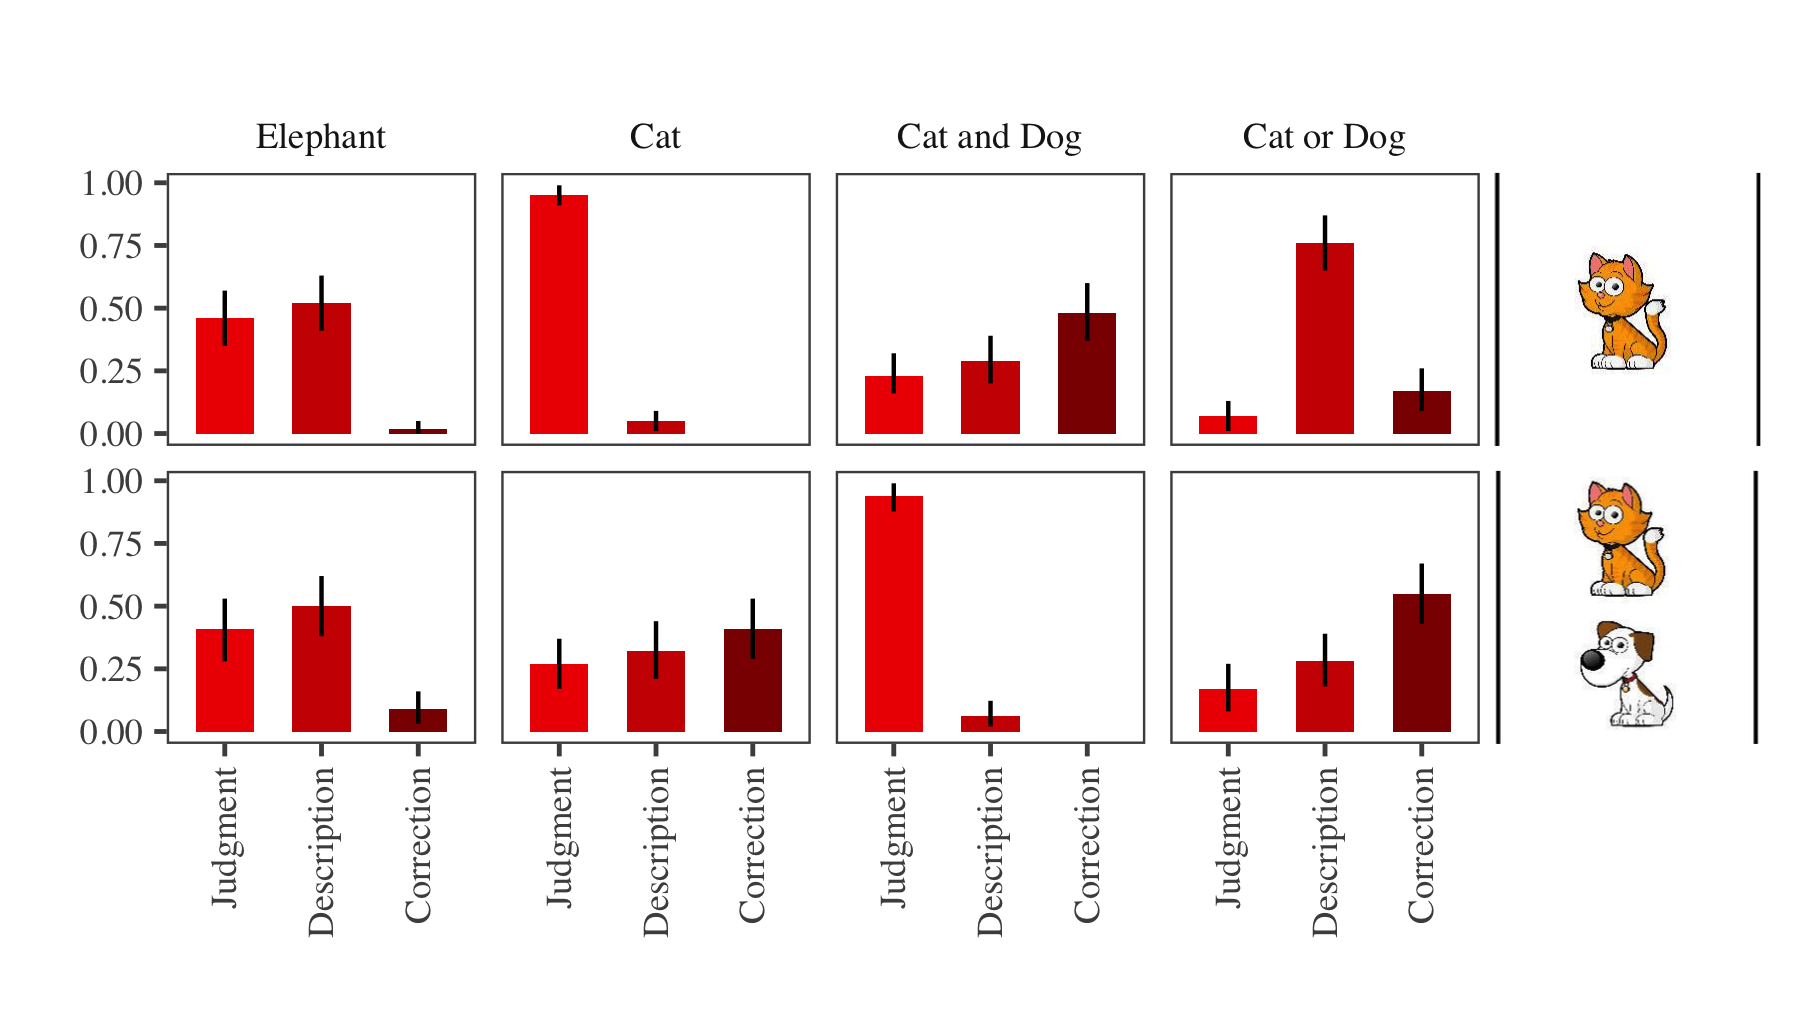
\includegraphics{figs/feedbackStudy3-1} 

}

\caption{Children's Open-ended Feedback in Study 3. Error bars represent 95\% confidence intervals.}\label{fig:feedbackStudy3}
\end{figure}

Figure \ref{fig:feedbackStudy3} shows the distribution of children's
feedback to the puppet in Study 3 (see Table \ref{tab:feedbackCat} for
the definitions and examples of feedback categories). There were no
\enquote{None} responses in this study since the experimenter explicitly
asked children to provide feedback to the puppet. The distribution of
the responses in the other three categories (Judgment, Description, and
Correction) revealed a successful replication of Study 2.

Children's feedback showed four main patterns. First when the puppet
guessed an animal not on the card (e.g.~elephant), there is a split
pattern between negative judgments like \enquote{no!} and simple
descriptions of what was on the card, e.g. \enquote{cat!}. Children
provided no corrections on such trials. Second, almost all children
responded with positive judgments like \enquote{yes} when the puppet's
guess accurately matched what was on the card. This was the case in
trials where there was only one animal on the card (e.g.~cat) and the
puppet mentioned it, as well as trials where there were two animals on
the card and the puppet mentioned both with a conjunction (e.g.~cat and
dog). Third, children provided the largest number of corrective feedback
in trials where the guess was either false or infelicitous. These
included three trial types: (a) the ones where there were two animals on
the card but the puppet only guessed one (e.g.~cat); (b) the ones where
the puppet guessed two animals with conjunction (e.g.~cat and dog) but
only one of them was on the card; and (c) the ones where there were two
animals on the card, and the puppet guessed both but used a disjunction
(e.g.~cat or dog). The fourth general pattern was unique to disjunctive
trials with only one animal on the card. In such cases, almost all
children simply named the animal on the card (e.g. \enquote{Cat!}).

\begin{figure}[t]

{\centering 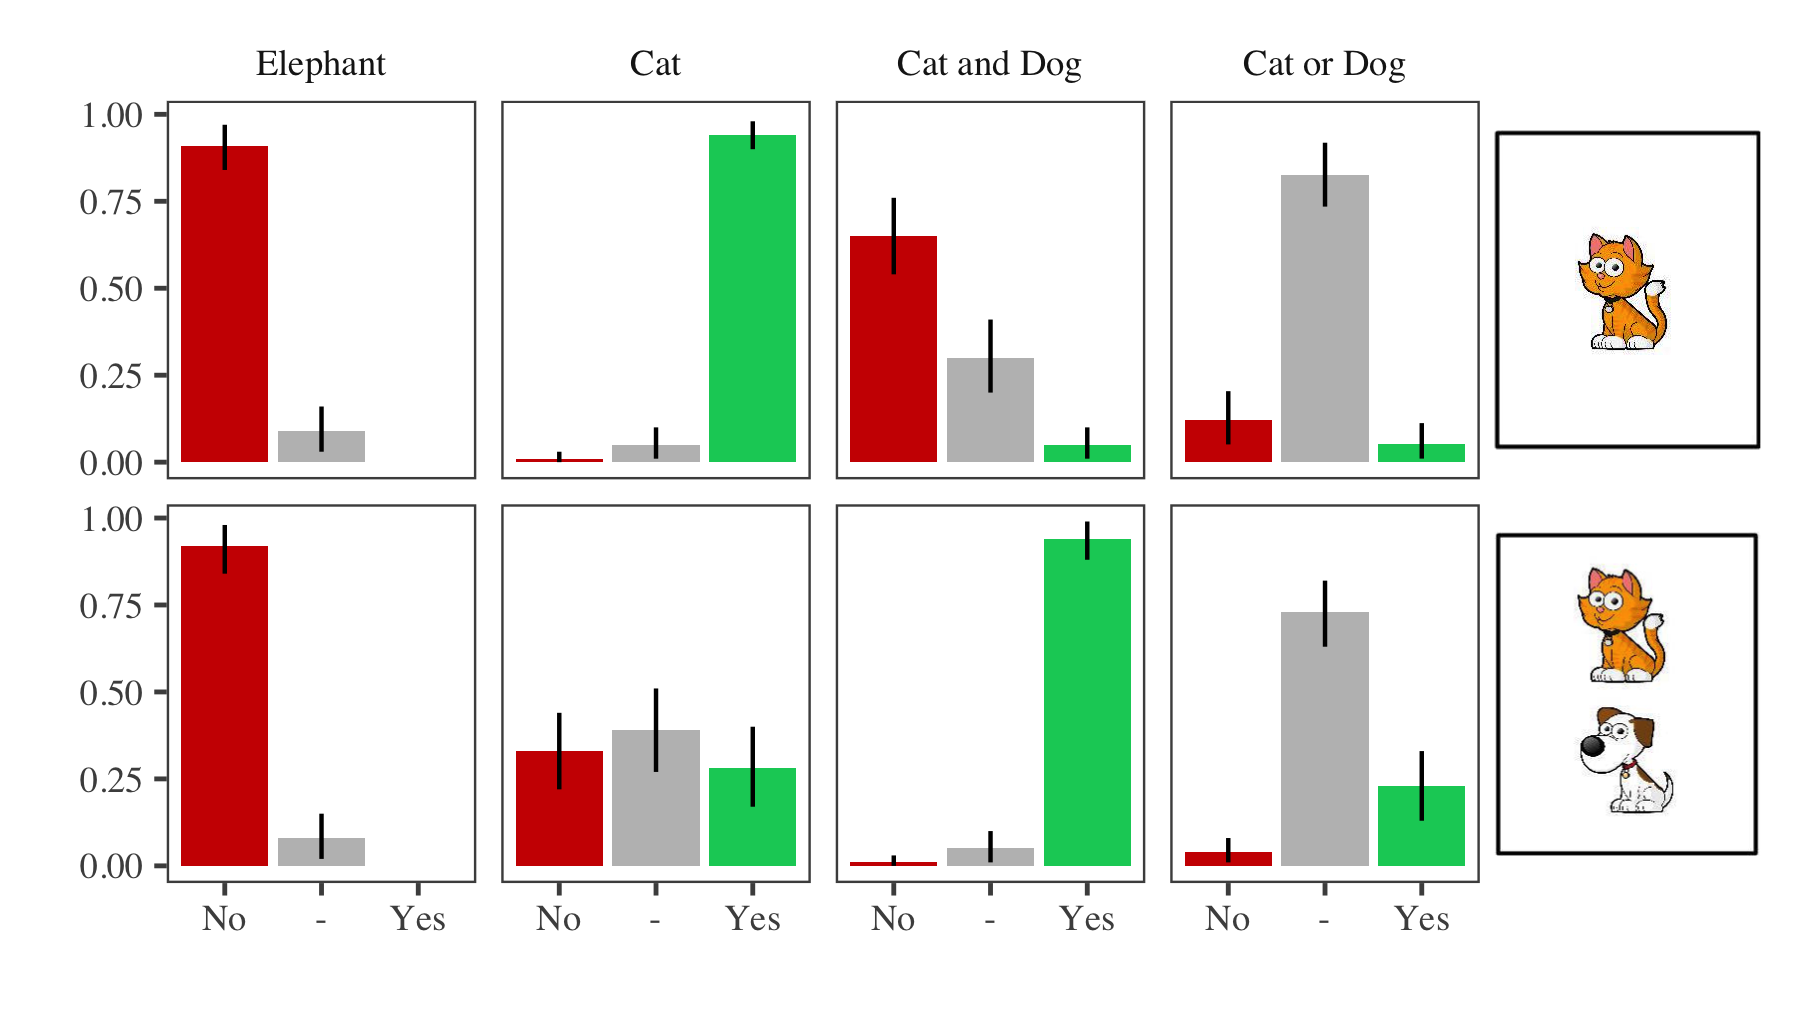
\includegraphics{figs/study3JudgmentPlot-1} 

}

\caption{Children's open-ended feedback to the puppet's guesses. The x-axis shows whether children spontaneously provided a yes (green), no (red), or other response (grey).}\label{fig:study3JudgmentPlot}
\end{figure}

Figure \ref{fig:study3JudgmentPlot} breaks down children's open-ended
feedback based on whether children said \enquote{yes}, \enquote{no}, or
said something else. Responses that were not \enquote{yes/no} judgments
are grouped in a middle category shown with a dash. The goal here is to
compare children's open-ended judgments with their forced choice
judgments shown in Figure \ref{fig:Study3tvjtPlot}. Children's
open-ended judgments and their forced choice judgments in study 3 show
similar patterns for all types of guesses except for disjunctive ones.
In trials that the puppet guessed with \emph{or}, the vast majority of
children refused to provide a \enquote{yes/no} judgment when they were
not forced to. Instead, they described the animal on the card or
provided corrections to the puppet's infelicitous disjunctive guess.

One way to interpret these results is that disjunctive guesses (with at
least one disjunct true) are considered neither right nor wrong by
almost all children. When children were forced to provide wrong-right
responses in the experimental context, some conformed to the adult
patterns of judgment and some did not. However, it is possible that such
deviations from adult judgments do not reflect differences in the
comprehension of disjunction, but rather differences in how children map
their adult-like comprehension onto the notions of \enquote{right} and
\enquote{wrong} in a forced choice judgment task. In other words, it is
possible that children and adults only differ in how they behave when
they are forced to respond with a fixed set of options.

\begin{figure}[t]

{\centering 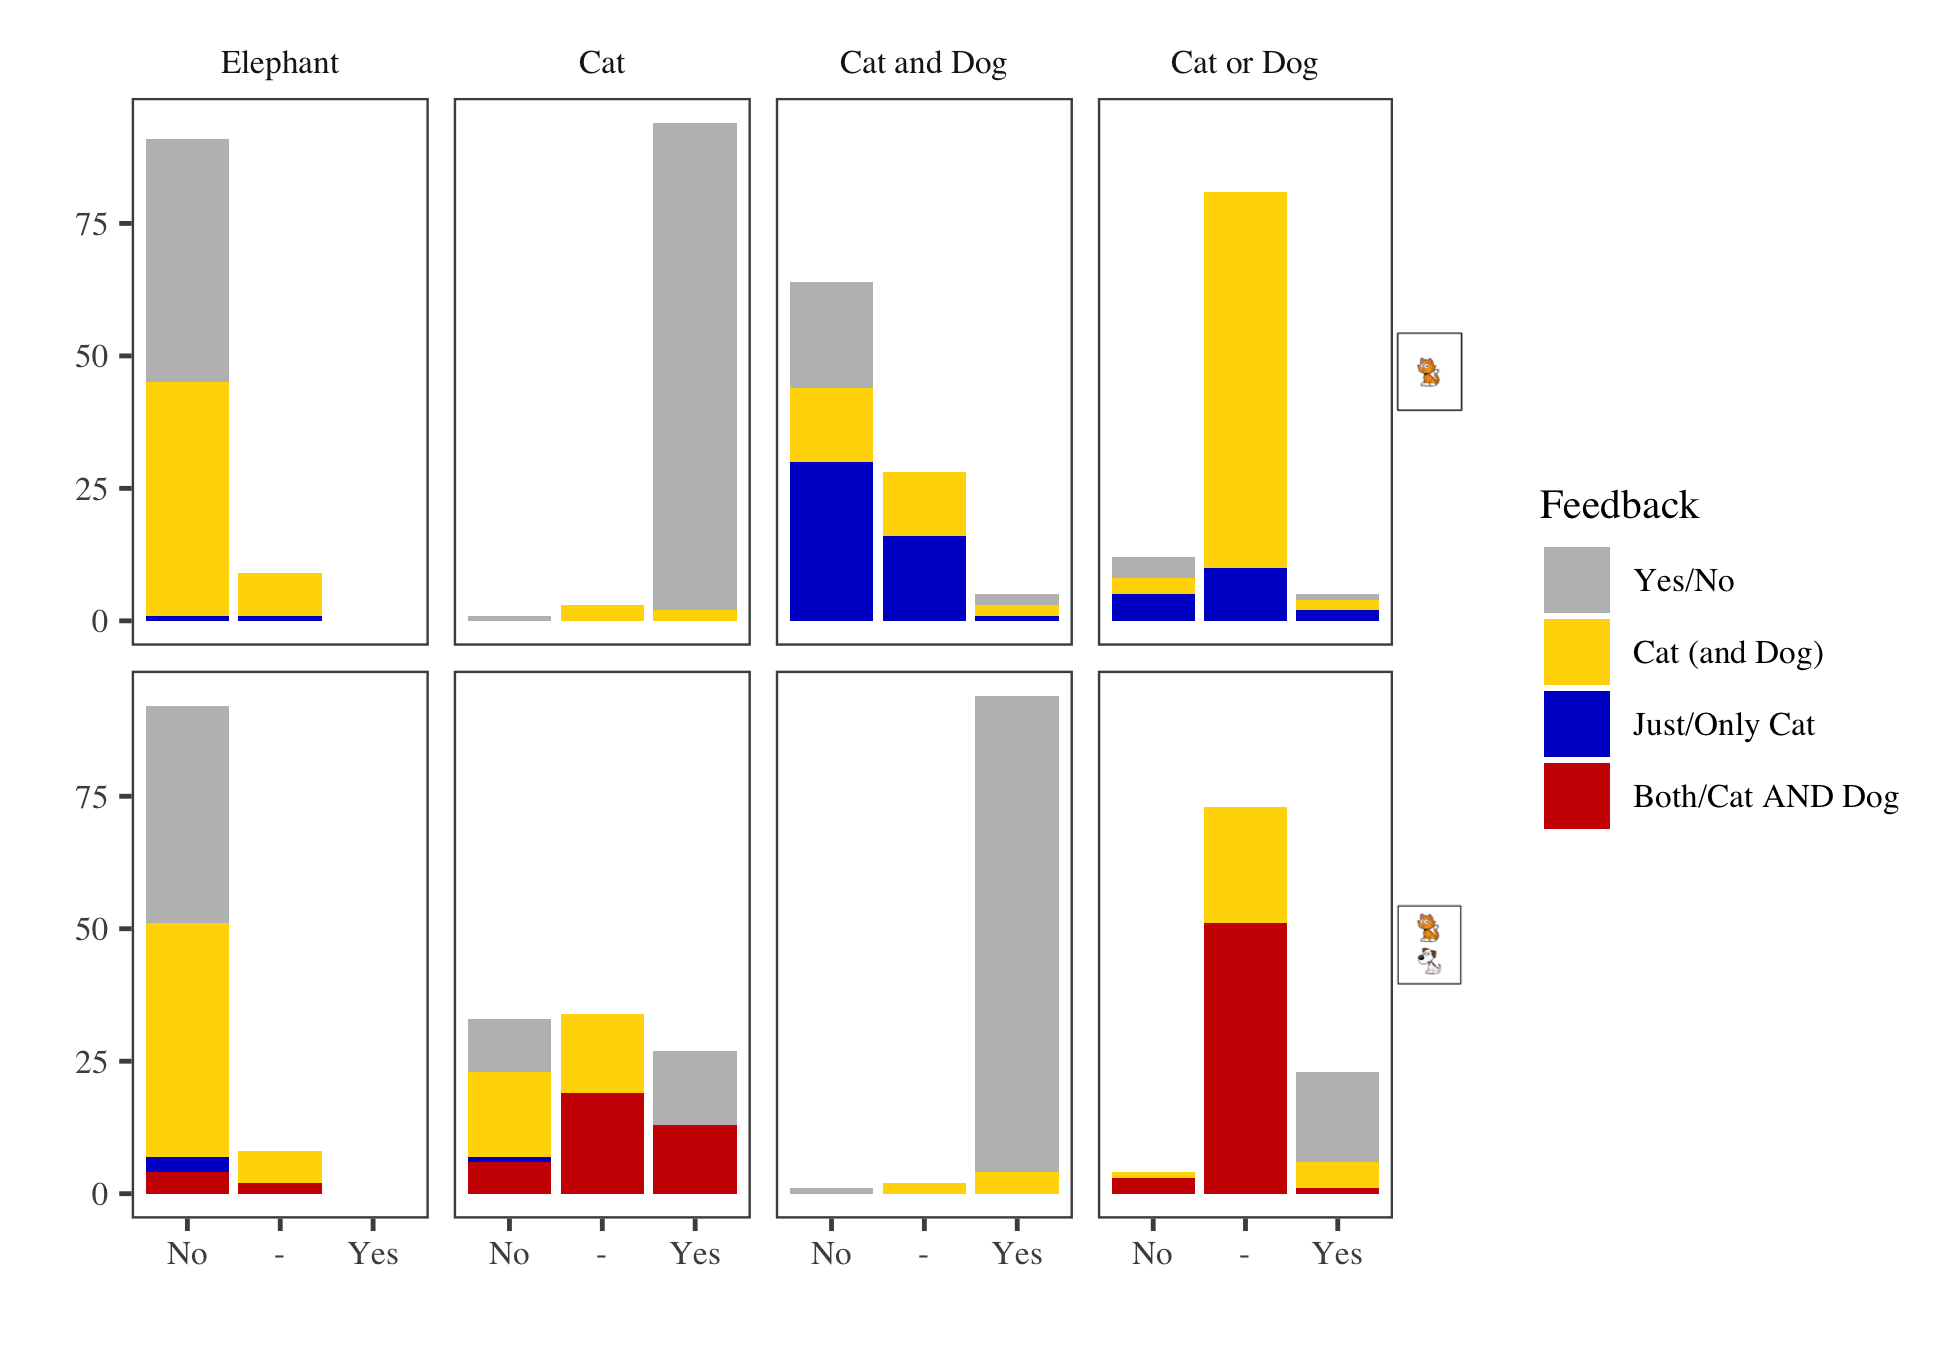
\includegraphics{figs/feedbackFillPlot-1} 

}

\caption{Children's open-ended feedback. The x-axis shows whether children said yes or no and the color fill shows what children said other than yes/no.}\label{fig:feedbackFillPlot}
\end{figure}

Figure \ref{fig:feedbackFillPlot} is similar to Figure
\ref{fig:study3JudgmentPlot} but it uses color-fill to show what
children said in addition to \enquote{yes/no}. The gray color represents
the trials where children only said \enquote{yes/no} and nothing else.
The yellow-fill represents descriptions where children mentioned the
animal on the card (e.g. \enquote{cat!}). The blue fill represents
children's corrective feedback that used the exclusive focus particles
\emph{just} or \emph{only} (e.g. \enquote{just a cat!}). Such a
corrective feedback suggests that the guess included an animal that did
not belong and should have been excluded. Finally the red fill
represents the inclusive corrective feedback that emphasized the word
\emph{and} or said \emph{both} (e.g. \enquote{Both!}, \enquote{cat AND
dog!}). Such corrective feedback indicated that both animals should have
been mentioned.

As shown in the leftmost column, when the puppet mentioned an animal
that was not on the card (e.g.~elephant), children responded with a
simple \enquote{no} or \enquote{no} followed by what was on the card
(e.g.~no! elephant!). When there was only one animal on the card and the
puppet mentioned the animal (e.g.~cat), children responded with a simple
\enquote{yes}. However, when the card had two animals (e.g.~cat and dog)
and the puppet only mentioned one of them (e.g.~cat), children were
likely to provide inclusive feedback. They said \emph{both} or
emphasized \emph{and}, as in \enquote{cat AND dog}. However, in such
trials children were equally split between saying \enquote{yes},
\enquote{no}, or neither.

In the trials with conjunctive and disjunctive guesses, when there was
only one animal on the card (e.g.~cat) and the puppet used a conjunction
(e.g.~cat and dog), children were likely to say a simple \enquote{no} or
say \enquote{no}, followed by \enquote{only/just} (e.g.~no, just a cat).
Some children did not say \enquote{no} but did respond with
\enquote{only/just}. When the card had two animals on it and the puppet
mentioned both using \emph{and}, children responded with a simple
\enquote{yes}. In trials with disjunctive guesses like \enquote{cat or
dog}, children avoided yes/no responses. Instead, when the card had only
one animal, children mentioned that animal. When the card had both
animals, children said \emph{both} or emphasized the word \emph{and}, as
in \enquote{cat AND dog}.

\begin{figure}[t]

{\centering 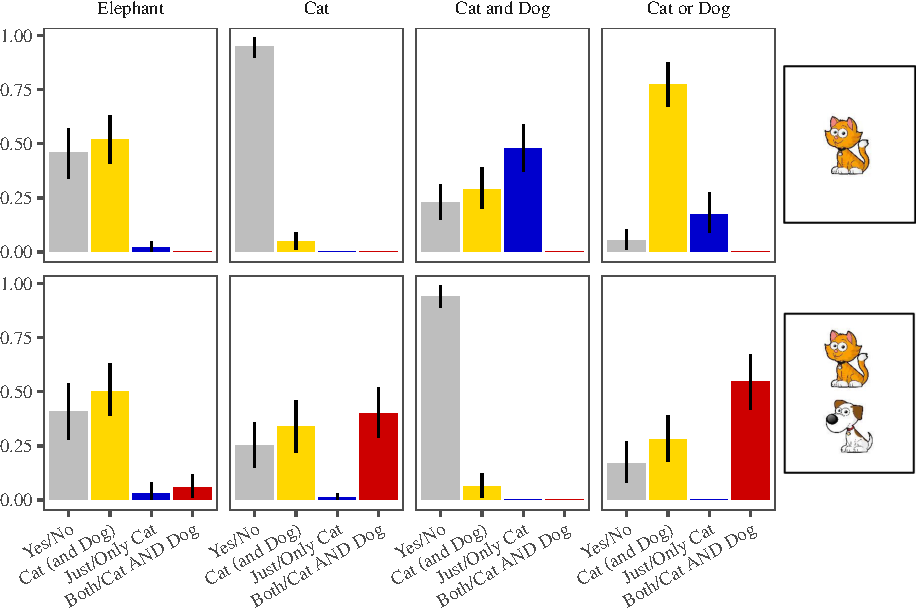
\includegraphics{figs/correctivePlot-1} 

}

\caption{Children's feedback categories in disjunction trials.}\label{fig:correctivePlot}
\end{figure}

Figure \ref{fig:correctivePlot} shows the same feedback data in Figure
\ref{fig:feedbackFillPlot} but uses the x-axis to also show the
proportion of feedback categories other than yes/no judgments. My goal
here is to display the trial types with corrective feedback (blue and
red). These trial types include: (1) conjunction when only one conjunct
is true, (2) disjunction when both disjuncts are true, and (3) simple
guesses (e.g. \enquote{there is a cat}) when two animals were on the
card. These trial types involved guesses that are either false or
infelicitous. Furthermore, the type of corrective feedback children
provided matched the type of mistakes made in the guesses. With
conjunctive guesses like \enquote{cat and dog} when there was only one
animal on the card (e.g.~cat), children provided exclusive corrections
(e.g.~just/only a cat), suggesting that the other animal (e.g.~dog)
should have been excluded. When two animals were on the card and the
puppet used a disjunctive guess like \enquote{cat or dog}, or simple
guess like \enquote{cat}, children provided inclusive feedback,
suggesting that another animal should have been included. This is
particularly notable in the case of disjunction since both animals were
mentioned, but children still emphasized that the connective \emph{and}
should have been used, or that both animals mentioned were on the card.

\subsubsection{Discussion}\label{discussion-2}

Study 3 measured children's comprehension of logical connectives by
asking them to judge a puppet's guess in two ways: with open-ended
feedback and with a two-alternative forced choice task. First, I asked
children to say \enquote{yes} to the puppet if he was right and
\enquote{no} if he was wrong. However, children could provide any form
of feedback they wanted. Second, I followed children's open-ended
feedback with a two-alternative forced choice question: \enquote{Was the
puppet right?} This way, I could measure children's comprehension in two
different ways in the same trial. Ideally, both measures should show
similar results. However, the findings were similar for conjunctive
guesses, but not disjunctive ones. Children avoided binary right/wrong
feedback with disjunction and preferred to provide more nuanced feedback
when they could.

The 2AFC responses followed the predicted pattern: conjunctive guesses
were judged wrong if only one conjunct was true, and right if both were
true. Disjunctive guesses were judged right whether one or both
disjuncts were true. There was no significant difference in the 2AFC
task between the responses of children and those of adults in Study 1.

Children's open-ended feedback in Study 3 replicated the findings of
Study 2. Children provided more corrective feedback in false and
infelicitous trials than in true and felicitous ones. The corrective
feedback was tailored to the puppet's mistake. If the puppet used a
conjunction when there was only one animal on the card, children pointed
out that the other animal should have been excluded using the exclusive
adverbials \emph{just} and \emph{only}. If the puppet used a disjunction
when both animals were on the card, children stressed \emph{and} or
\emph{both}, implying that both animals should be included.

While the 2AFC results suggested that children take no issue with
disjunctive guesses when both disjuncts are true, the analysis of their
corrective feedback showed that they provide appropriate corrections in
such cases and emphasize that the connective \emph{and} would have been
a better guess. Taking both measures together, I conclude that even
though children are aware of the problem with such guesses, they do not
consider them \emph{wrong}. These results are similar to those I
reported for adults in Study 1.

\subsection{General Discussion}\label{general-discussion}

I reported three studies on adults and four-year-olds' comprehension of
the logical connectives \emph{and} and \emph{or}. The first study used
two- and three-alternative forced choice judgment tasks with adults. In
the 2AFC task, adult interpretations closely matched the semantic
accounts of \emph{and} and \emph{or} as conjunction and inclusive
disjunction. The judgments did not register robust signs of pragmatic
infelicities. However, the 3AFC judgment task, showed signs of pragmatic
infelicities, especially in disjunctive guesses with true disjuncts.
When both disjuncts were true, participants were more likely to choose
\enquote{kinda right} rather than \enquote{right}.

The second study used a 3AFC judgment task with four-year-old children.
It also included an exploratory analysis of children's open-ended verbal
feedback to the puppet in the experimental setting. Children's
interpretations were similar to those of adults in the 3AFC task and
only differed for pragmatically infelicitous disjunctions. When both
disjuncts were true, adults tended to judge disjunctive guesses as
\enquote{kinda right}. This was evidence for the pragmatic infelicity of
such guesses. While, children judged such disjunctive statement as
\enquote{right}, the analysis of their open-ended feedback showed that
they took issue with such statements as well, and provided appropriate
corrective feedback.

In the third study, I focused on eliciting open-ended verbal feedback
from children and followed it with a 2AFC task. In the 2AFC task,
children's responses reflected the semantics of connectives as
conjunction and inclusive disjunction. There was no significant
difference between children and adults in the two-alternative judgments.
Since the 2AFC task appeared to be a good indicator of semantic
knowledge, it seemed reasonable to conclude that adults and
four-year-olds displayed similar semantic knowledge of the connectives.
Analysis of the children's open-ended feedback replicated the findings
in study 2. Children provided more corrective feedback in false and
pragmatically infelicitous trials with logical connectives than in
felicitous trials. The comparison of the 2AFC task and children's
open-ended responses shows that children are sensitive to the infelicity
of disjunctions with true disjuncts, even though they consider them to
be \enquote{right} guesses.

Overall, I did not find any major differences between adults' and
four-year-old children's interpretations of logical connectives
\emph{and} and \emph{or} in the context of the guessing game. However,
there were two minor differences. First, I found that in both 2AFC and
3AFC judgment tasks, children showed a small preference for disjunctions
with both disjuncts true rather than only one. Adults on the other hand
showed the opposite pattern: they preferred disjuncts with only one
disjunct true. Second, in both 2AFC and 3AFC judgment tasks, children
rated disjunctions with both disjuncts true higher than adults did. That
is, they considered utterances like \enquote{there is a cat or a dog}
when both animals were on the card \enquote{right} more often than
adults. Here I will discuss these two differences and their possible
causes in more detail.

\subsubsection{Preference for True Disjuncts}\label{conjunctive}

First for some children, there was a small preference for both disjuncts
being true, compared to only one. This effect is similar in kind but not
magnitude, to an effect that Singh et al. (2016) and Tieu et al. (2016)
reported. In my study this effect is quite small while Singh et al.
(2016) and Tieu et al. (2016) seem to have found bigger effects. Based
on this, Singh et al. (2016) proposed that many children at this
age-range have a pragmatically driven conjunctive interpretation of
disjunction. In short, due to a non-adult like alternative set to the
connective \emph{or}, children strengthen a disjunctive statement
pragmatically and derive a conjunction. The studies reported here
provide no support for this proposal. In both 2AFC and 3AFC judgments,
children clearly differentiated between disjunctive and conjunctive
guesses. Furthermore, analysis of children's open-ended feedback showed
distinctly different response patterns for conjunction and disjunction.
More importantly, the open-ended feedback to disjunctive guesses showed
the opposite pattern to that predicted by the conjunctive hypothesis.
Children took issue with disjunctions that had both disjuncts true and
provided more corrective feedback in such cases. Therefore, the findings
from Singh et al. (2016) and Tieu et al. (2016) appear to be a product
of experimental design rather than a real reflection of children's
comprehension of the connectives.

However, even if this small preference for true disjuncts is not due to
the method of measurement, it can be accounted for in several other ways
that have not yet been successfully ruled out. First, the conjunctive
interpretation may not be due to a faulty pragmatic computation, but
rather a default conjunctive interpretation when the connective is not
properly heard, understood or is unknown. To check this hypothesis, it
should be possible to test children's comprehension of novel or noisy
connectives. A novel coordination like \emph{cat dax dog} with
\emph{dax} as a nonce connective could well be interpreted as a
conjunction. Such a result would suggest that in studies with high
cognitive demand, children may default to a conjunctive interpretation
if they miss the relevant connective. Second, the conjunctive preference
could be due to some children's preference for the linguistic labels to
match the animals on the card (or more generally a match between
linguistic description and the state of the world). This hypothesis is
consistent with the results in the other trial type that had a mismatch
in the number of animals and the guess, where the guess was still
technically true: simple guesses (e.g.~there is a cat) with two animals
(e.g.~cat and dog). Children were equally split between \enquote{wrong}
and \enquote{right} in their judgments here, while adults considered
such guesses \enquote{right}. In light of these alternative
explanations, I am hesitant to attribute this small preference to a
pragmatically driven conjunctive interpretation of disjunction.

\subsubsection{Lack of Infelicity with True
Disjuncts}\label{lack-of-infelicity-with-true-disjuncts}

The second difference between adults and children emerged in the 3AFC
judgment task: in disjunctive trials (e.g. \enquote{cat or dog}) with
two animals (e.g.~cat and dog), adults were more likely to choose
\enquote{kinda right} than children were. Children mostly chose
\enquote{right}. This response pattern has been taken to mean that
children found no infelicity with such disjunctions or that they did not
\enquote{derive an exclusivity implicature}. The absence of an
infelicity/implicature is consistent with the generalization that
children are more likely than adults to interpret scalar terms
literally, and that children do not compute implicatures or judge
infelicity to the same \textbf{rate} that adults do (Pouscoulous \&
Noveck, 2009, Katsos (2014)). But why is that?

There have been three major proposals to account for children's low rate
of implicatures: 1. processing (Pouscoulous, Noveck, Politzer, \&
Bastide, 2007; Reinhart, 2004) 2. non-adult-like lexical entry (Barner
et al., 2011; Horowitz, Schneider, \& Frank, 2017) and 3. pragmatic
tolerance (Katsos \& Bishop, 2011). Here I show that none of these
accounts can provide a satisfactory explanation of the results in this
study.

\textbf{1. Processing.} First, the processing accounts locate the
problem in children's processing capacities such as working memory. They
suggest that pragmatic computations are cognitively taxing and children
lack the appropriate processing resources to carry them out
appropriately. A prediction of processing accounts (at least in their
current format) is that children will show reduced implicature
computations for all types of implicatures -- scalar or ad-hoc. This
prediction was not borne out in my experimental results. In Study 3,
children were much more likely than adults to call a simple guess (e.g.
\enquote{cat}) \enquote{wrong} in the 2AFC task if there were two
animals on the card (e.g. \enquote{cat and dog}). Processing accounts do
not predict that children would derive more implicatures than adults but
this is what I found for the traditional interpretation of the judgment
task.

\textbf{2. Non-adult-like Lexicon.} Several proposals blame the
structure of the child's lexicon for the alleged failure in deriving
implicatures. The assumption is that the child's lexical entry for
scalar items must include three elements for successful derivation: 1.
the semantics of the weak term (e.g. \emph{some}, \emph{or}) 2. the
semantics of the strong term (e.g. \emph{all},\emph{and}); and possibly
3. a scale that recognizes the stronger term as an alternative to the
weaker one (e.g. \textless{}\emph{some}, \emph{all}\textgreater{},
\textless{}\emph{or}, \emph{and}\textgreater{}). Each of these elements
have been pinpointed as the source of the problem in previous studies
(Barner et al., 2011; Horowitz et al., 2017; Katsos \& Bishop, 2011).
However none of them seem to apply to the results reported here.

If children in this study lack the semantics of the connective
\emph{or}, I would expect them to either perform at chance or default to
a conjunctive interpretation. Neither prediction was borne out in
studies 2 and 3. Furthermore, children's free-form linguistic feedback
suggests good understanding of disjunction. So this explanation seems
unlikely. The problem cannot be that children do not know the meaning of
\emph{and} either. Children's performance in both study 2 and 3 for
conjunction trials show that they understand its meaning very well.
Finally, while it is possible that children lacked the appropriate
lexical scale and could not access the stronger alternative, this
explanation cannot be the whole story. Several children in both studies
stressed the word \emph{and} suggesting that the puppet should have used
the stronger term instead. However, they judged the puppet's guess as
\enquote{right}. If children could not access the stronger term, they
would not have mentioned it in their feedback either.

\textbf{3. Pragmatic Tolerance.} Katsos \& Bishop (2011) suggested that
children tend to tolerate pragmatic infelicities more than adults. They
showed that when children are provided with a 2AFC judgment task, they
tolerate the infelicity of \emph{some} when \emph{all} applies but when
they are presented with a 3AFC task they choose the middle option and
report this infelicity. As in a processing account, the pragmatic
tolerance account predicts that scalar and ad-hoc implicatures will be
similarly affected. However, my results did not match those of Katsos \&
Bishop (2011). When children were presented with a 3AFC task, they chose
the highest reward (and not the middle option) for uses of \emph{or}
when \emph{and} applied. Second, and more importantly, I found different
patterns for ad-hoc and scalar implicatures as mentioned before. This is
not predicted by the tolerance account unless children are assumed to be
more tolerant towards violations of scalar implicatures than they are
towards ad-hoc ones. While tolerance may not be the source of the
problem here, I believe that a number of discussions including those by
Katsos \& Bishop (2011) and later Katsos (2014) do point to an important
factor: the role of measurement in estimates of children's pragmatic
capacity.

Several observations in the current studies provide support for the
hypothesis that methodological issues, and more specifically issues of
measurement contribute to the differences found between adults and
children in pragmatic capacity. First, Study 1 showed that even for
adults, the estimates of adult infelicity rates may differ based on the
number of alternatives in the forced choice task. A 2AFC task tends to
underestimate adults' rate of response to pragmatic infelicity. Second,
children's open-ended linguistic feedback in the experimental context
better reflected their sensitivity to pragmatic nuances than the
forced-choice judgment tasks. Third, children showed a higher rate of
infelicity judgments for cases of ad-hoc implicatures (simple guesses
with two animals on the card) than adults did. While a difference in
sensitivity to ad-hoc vs.~scalar implicatures has been reported and
argued for before (Horowitz et al., 2017; Stiller, Goodman, \& Frank,
2015), a higher sensitivity than adults is not predicted by any of the
current accounts.

In order to better understand the differences between adults and
children's pragmatic capacities, it is necessary to have a good
understanding of how measurements affect estimates of adults and
children's performance in the experimental tasks. Children may be no
more capable of making exhaustive inferences than adults and no less
capable of making scalar inferences either. They may simply have a
different construal of the wrong-right scale and of what the
forced-choice task is about. The concepts \enquote{right} and
\enquote{wrong} are as much subject to developmental change and
differences between adults and children as are scalar items in general.
It is reasonable to assume that children's understanding of what
constitutes as \enquote{right} or \enquote{wrong} does not fully conform
to that of adults. However, it remains to be established what these
differences are and how they affect the estimates of children's
pragmatic abilities. It is important to point out that such issues of
measurement could be the culprit behind both children's seemingly slight
preference for true disjuncts described earlier and the lack of
infelicity judgments when both disjuncts are true.

\textbf{A General Approach for Measuring Implicature/Infelicity Rate}

Methodological issues are nothing new in studies of children's semantic
and pragmatic development. Developing better measures of children's
linguistic capacities has always been a major concern for researchers in
the field. My goal here is to propose some future steps that can address
the methodological concerns in measuring children's pragmatic
development.

As Pouscoulous \& Noveck (2009) and Katsos (2014) have suggested, the
central issue is \enquote{the rate} at which children and adults
manifest pragmatic reasoning in the experimental setting. No one doubts
children's capacity to perform such computations. At issue is the extent
to which children and adults compute specific implicatures. The claims
are that children perform such computations less often than adults; or
that children do not perform such computations where adults normally do.
In the previous section, I discussed some factors that might account for
these differences including processing demands, the structure of the
lexicon, tolerance, as well as issues of measuring adults and children's
comprehension. As Katsos (2014) pointed out, it seems reasonable to
assume that all these factors play some part here. What matters is the
degree to which each contributes to the outcome.

\begin{figure}[t]

{\centering 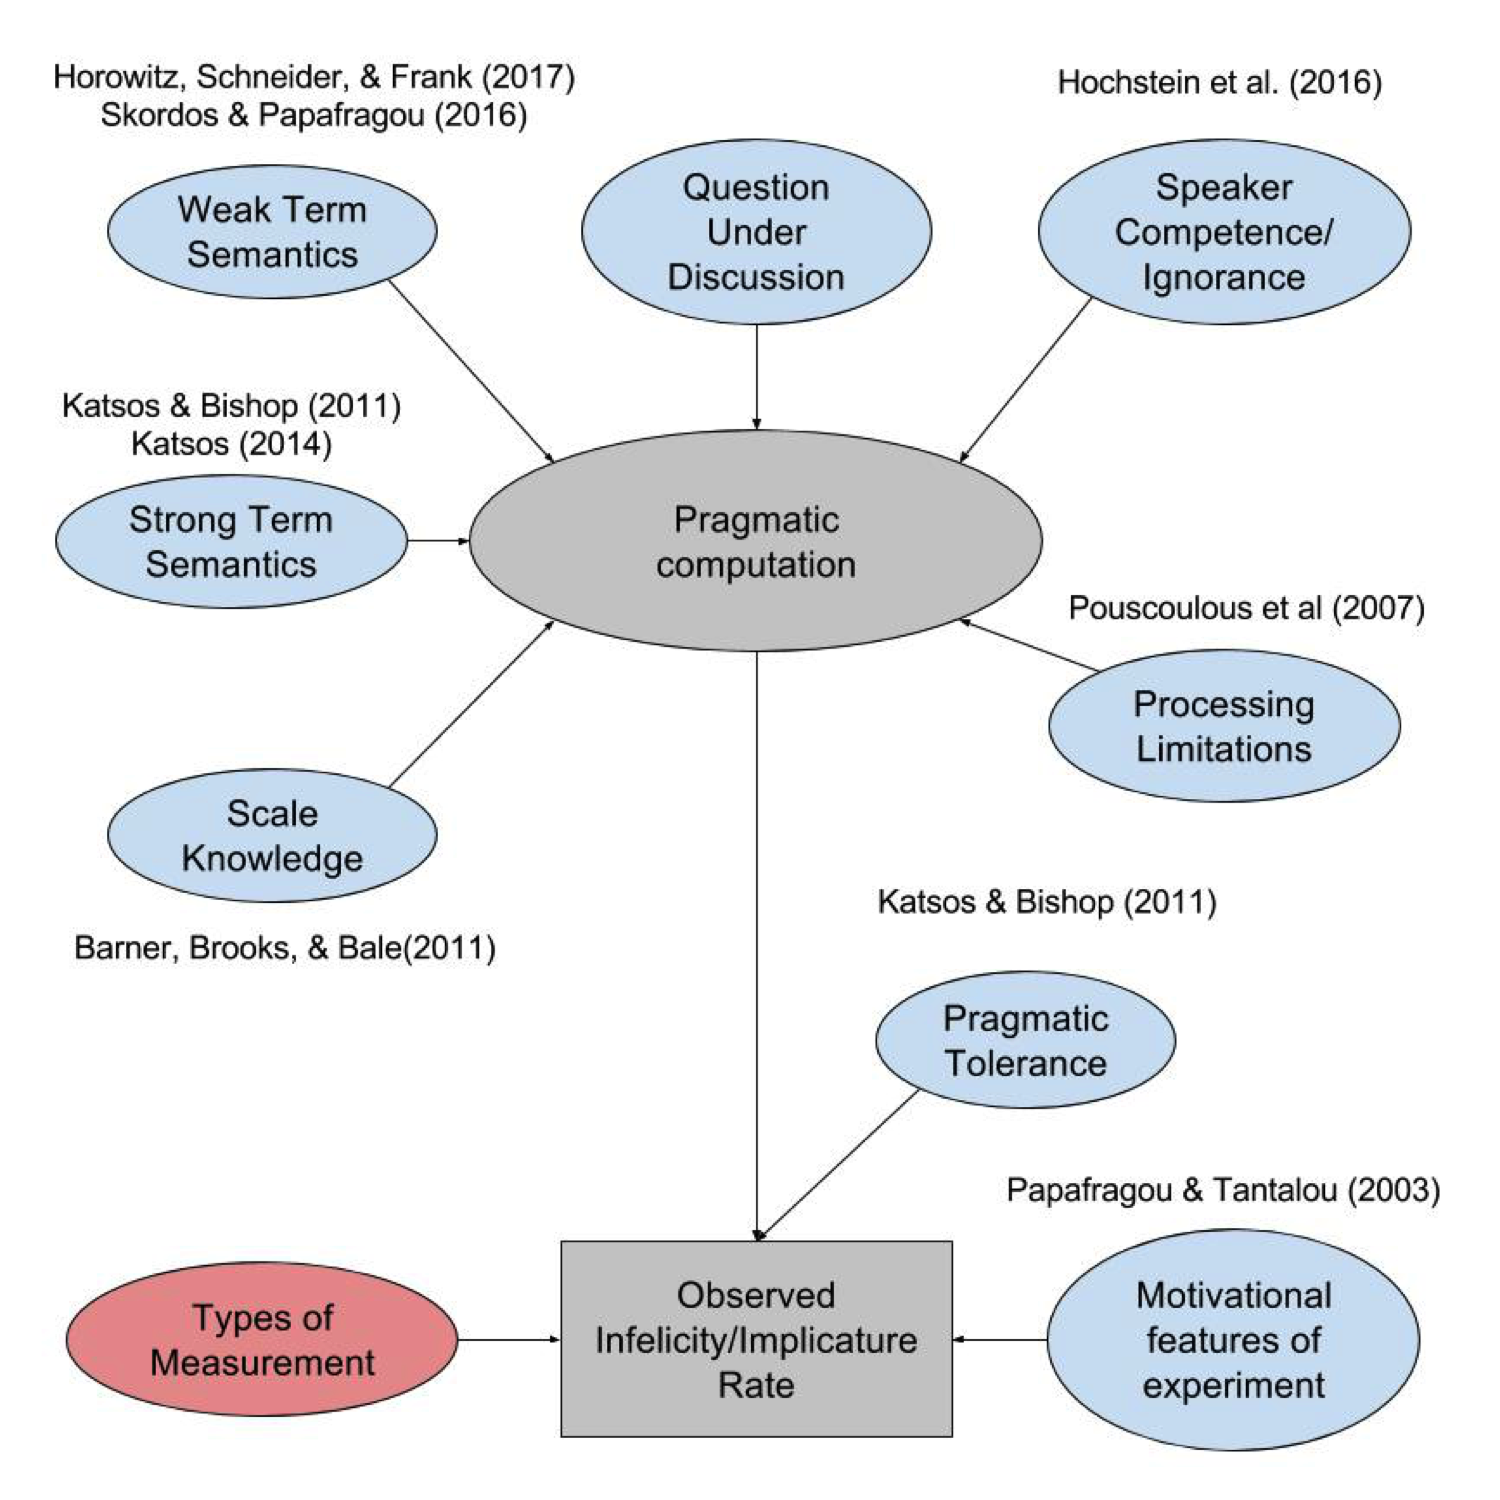
\includegraphics{figs/implicatureGraph-1} 

}

\caption{Factors that could affect pragmatic computations and the estimates of these computations in the experimental settings}\label{fig:implicatureGraph}
\end{figure}

Figure \ref{fig:implicatureGraph} shows the factors that affect
pragmatic computations as well as the observations of the rate of
pragmatic computations in an experiment. First it is important to
distinguish between factors that affect pragmatic computations and those
that affect the observed rate in an experimental setting. As I showed in
Study 1, given the number of alternatives in the forced choice task
(2AFC vs.~3AFC), I may get different estimates of adults' infelicity
judgments, yet it is unreasonable to assume that there is a difference
in adults' pragmatic capacities in these two tasks. A similar situation
exists when I compare children's forced choice measures of infelicity
and their open-ended feedback. In disjunctive trials where both
disjuncts are true, the forced choice tasks show no sign of children
detecting infelicity while the open ended responses show that children
are sensitive to the infelicity of disjunction when a conjunction would
have been more appropriate.

\subsection{Conclusion}\label{conclusion}

To conclude, I have shown that children and adults do not differ
substantially in their \textbf{semantic} knowledge of the logical
connectives \emph{and} and \emph{or}. The results were highly consistent
with the current accounts that posit the semantics of \emph{and} as
logical conjunction and \emph{or} as logical (inclusive) disjunction.
With respect to pragmatic knowledge, the three-alternative forced choice
judgment task showed that adults are sensitive to the infelicity of
disjunctive statements when both disjuncts are true. I also showed that
while the three-alternative judgment task failed to register such a
sensitivity for children, my systematic analysis of children's verbal
open-ended verbal feedback showed that children are sensitive to
pragmatic infelicities and can provide appropriate corrections to
infelicitous utterances containing logical connectives.

\newpage

\section{References}\label{references}

\setlength{\parindent}{-0.5in} \setlength{\leftskip}{0.5in}

\hypertarget{refs}{}
\hypertarget{ref-Aloni2016}{}
Aloni, M. (2016). Disjunction. In E. N. Zalta (Ed.), \emph{The Stanford
encyclopedia of philosophy}. Stanford University. Retrieved from
\url{https://plato.stanford.edu/archives/win2016/entries/disjunction/}

\hypertarget{ref-barner2011accessing}{}
Barner, D., Brooks, N., \& Bale, A. (2011). Accessing the unsaid: The
role of scalar alternatives in children's pragmatic inference.
\emph{Cognition}, \emph{118}(1), 84--93.

\hypertarget{ref-braine1981development}{}
Braine, M. D., \& Rumain, B. (1981). Development of comprehension of
``or'': Evidence for a sequence of competencies. \emph{Journal of
Experimental Child Psychology}, \emph{31}(1), 46--70.

\hypertarget{ref-crain2012emergence}{}
Crain, S. (2012). \emph{The emergence of meaning}. Cambridge: Cambridge
University Press.

\hypertarget{ref-crain1998investigations}{}
Crain, S., \& Thornton, R. (1998). \emph{Investigations in universal
grammar: A guide to experiments on the acquisition of syntax and
semantics}. Cambridge, MA: MIT Press.

\hypertarget{ref-gazdar79}{}
Gazdar, G. (1979). \emph{Pragmatics: Implicature, presupposition, and
logical form}. New York: Academic Press.

\hypertarget{ref-grice1989studies}{}
Grice, H. P. (1989). \emph{Studies in the way of words}. Cambridge, MA:
Harvard University Press.

\hypertarget{ref-gutzmann2014}{}
Gutzmann, D. (2014). Semantics vs. pragmatics. In L. Matthewson, C.
Meier, H. Rullmann, \& T. E. Zimmermann (Eds.), \emph{The companion to
semantics}. Oxford: Wiley.

\hypertarget{ref-horn1989natural}{}
Horn, L. (1989). \emph{A natural history of negation}. Chicago, IL:
University of Chicago Press.

\hypertarget{ref-horowitz2017trouble}{}
Horowitz, A. C., Schneider, R. M., \& Frank, M. C. (2017). The trouble
with quantifiers: Exploring children's deficits in scalar implicature.
\emph{Child Development}.

\hypertarget{ref-jasbiWaldonDegan2017}{}
Jasbi, M., Waldon, B., \& Degen, J. (submitted). \emph{Linking
hypothesis and number of response options modulate inferred scalar
implicature rate}.

\hypertarget{ref-katsos2014scalar}{}
Katsos, N. (2014). Scalar implicature. In D. Matthews (Ed.),
\emph{Pragmatic development in first language acquisition} (Vol. 10, p.
183---198). Amsterdam: John Benjamins.

\hypertarget{ref-katsos2011pragmatic}{}
Katsos, N., \& Bishop, D. V. (2011). Pragmatic tolerance: Implications
for the acquisition of informativeness and implicature.
\emph{Cognition}, \emph{120}(1), 67--81.

\hypertarget{ref-noveck2001children}{}
Noveck, I. A. (2001). When children are more logical than adults:
Experimental investigations of scalar implicature. \emph{Cognition},
\emph{78}(2), 165--188.

\hypertarget{ref-pouscoulous2009going}{}
Pouscoulous, N., \& Noveck, I. A. (2009). Going beyond semantics: The
development of pragmatic enrichment. In S. Foster-Cohen (Ed.),
\emph{Language acquisition} (pp. 196--215). Berlin: Springer.

\hypertarget{ref-pouscoulous2007developmental}{}
Pouscoulous, N., Noveck, I. A., Politzer, G., \& Bastide, A. (2007). A
developmental investigation of processing costs in implicature
production. \emph{Language Acquisition}, \emph{14}(4), 347--375.

\hypertarget{ref-reinhart2004processing}{}
Reinhart, T. (2004). The processing cost of reference set computation:
Acquisition of stress shift and focus. \emph{Language Acquisition},
\emph{12}(2), 109--155.

\hypertarget{ref-Singh2016}{}
Singh, R., Wexler, K., Astle-Rahim, A., Kamawar, D., \& Fox, D. (2016).
Children interpret disjunction as conjunction: Consequences for theories
of implicature and child development. \emph{Natural Language Semantics},
\emph{24}(4), 305--352.

\hypertarget{ref-stiller2015ad}{}
Stiller, A. J., Goodman, N. D., \& Frank, M. C. (2015). Ad-hoc
implicature in preschool children. \emph{Language Learning and
Development}, \emph{11}(2), 176--190.

\hypertarget{ref-tieu2016}{}
Tieu, L., Yatsushiro, K., Cremers, A., Romoli, J., Sauerland, U., \&
Chemla, E. (2016). On the role of alternatives in the acquisition of
simple and complex disjunctions in french and japanese. \emph{Journal of
Semantics}.






\end{document}
